\chapter{Results}
\label{cha:results}

 
Chapter~\ref{cha:method} asserted a segmentation rule, a churn threshold, an interval width and a covariate set. This chapter supplies the evidence for each in that order, before turning to the fitted models in Section~\ref{sec:res-models}.
 
\section{The estimation sample (LOOKS GOOD)}
\label{sec:res-attrition}
\label{sec:res-segmentation}
\label{sec:res-activity-mix}


 \begin{table}[htbp]
\centering
\small
\begin{tabular}{@{}lrr@{}}
\toprule
& Personal & Professional \\
\midrule
After segmentation \eqref{eq:segmentation-rule} & 8{,}328 & 579 \\
After the inactivity rule, censoring and entry filter & 6{,}000 & 514 \\
Removed & 2{,}328 & 65 \\
\addlinespace
Events    & 2{,}774 & 254 \\
Censored  & 3{,}226 & 260 \\
Customers with an event & 46.2\% & 49.4\% \\
\addlinespace
Person-interval rows & 124{,}783& --- \\
Rows carrying an event & 2.22\% & --- \\
\bottomrule
\end{tabular}
\caption{Customers before and after the restrictions of Section~\ref{sec:sample-restriction}. The restrictions are applied jointly, so the counts are not sequential. The professional segment is shown for comparison and is not modelled.}
\label{tab:attrition}
\end{table}
 
The restrictions of Section~\ref{sec:sample-restriction} -- the inactivity rule, the cutoff-minus-$\theta$ censoring and the 56-day entry filter -- cost the personal segment 2{,}328 of the 8{,}328 customers the segmentation rule assigned to it, or 27.9\% (Table~\ref{tab:attrition}). The 6{,}000 that survive contribute 124{,}783 person-interval rows. Just under half of them churn, and 2.22\% of rows carry the event.

 
Every \texttt{vehicle\_id} in the activity log matches a row in the vehicle table, so the right join of Section~\ref{sec:joining} loses no activity. What it cannot reach is the 7{,}762 activity rows that carry no \texttt{vehicle\_id} at all. \texttt{vehicle\_end\_year} is missing for 7.31\% of vehicles, which is the share treated as still in production. Five customers held a single \texttt{vehicle\_id} against conflicting metadata and all of their data was completely dropped.
 
Condition C of~\eqref{eq:segmentation-rule} needs a cut-off $q$ on distinct vehicles per customer. The 90th percentile of that count sets it at 11; across all merged customers the 95th percentile is 20.
 
Figure~\ref{fig:user-split} plots each customer by distinct vehicle count against top-four vehicle share, with point size giving the effective vehicle count, and the two segments separate on both axes at once. Personal customers run from 1 to 115 distinct vehicles, hold top-four shares between 0.44 and 1.00, and never exceed an effective count of 10.0. Professional customers reach 1{,}347 distinct vehicles, top-four shares as low as 0.05, and effective counts in the hundreds. The largest has an effective count of 226, more than twenty times anything in the personal segment.
 
\begin{figure}[htbp]\centering
\includegraphics[width=\textwidth]{Images/02_user_split_validation.png}
\caption{Customers by distinct vehicle count and top-four vehicle share, sized by effective vehicle count. The horizontal scales differ.}
\label{fig:user-split}
\end{figure}
 
The two groups use the app very differently. Diagnostic scans take 238{,}049 of the 482{,}354 personal actions, 49.4\% of the total, and no other activity reaches 12\%. Among professionals scans fall to 40.5\% of 102{,}176 actions while one-click apps rise from 9.2\% to 24.6\% and manual coding from 7.8\% to 14.2\% (Figure~\ref{fig:activity-mix}). The segmentation rule uses vehicle counts and never touches the activity log, so the split it produces is related to the behaviour it did not see. The six modelled activity groups cover 93.1\% of personal actions and 98.0\% of professional ones. What remains is led by car alerts at 3.9\% of personal activity and tails off to 177 maintenance reminders and 28 battery checks.
 
\begin{figure}[htbp]\centering
\includegraphics[width=\textwidth]{Images/01_activity_type_distribution.png}
\caption{Activity types by segment, with counts and shares. Personal above, professional below. The vertical scales differ.}
\label{fig:activity-mix}
\end{figure}
 
The professional segment appears in Table~\ref{tab:attrition} for comparison only. Its event count is too few to support a 27-covariate model, by the margin Section~\ref{sec:res-epv} sets out. That is what keeps it out of the analysis. Everything below is the personal segment, and the first thing its 6{,}000 customers need is a definition of churn.
 
\section{How long an absence has to be for churn (LOOKS GOOD)}
\label{sec:res-gaps}
\label{sec:res-seasonality}
 
\begin{table}[htbp]
\centering
\small
\begin{tabular}{@{}lrr@{}}
\toprule
Statistic & Personal & Professional \\
\midrule
Count & 172{,}331 & 35{,}324 \\
Mean  & 18.4 & 8.5 \\
SD    & 41.3 & 17.4 \\
Minimum & 1 & 1 \\
25th percentile & 1 & 1 \\
Median & 4 & 3 \\
75th percentile & 15 & 8 \\
90th percentile & 47 & 20 \\
95th percentile & 86 & 33 \\
99th percentile & 213 & 83 \\
Maximum & 937 & 425 \\
\bottomrule
\end{tabular}
\caption{Days between consecutive active days by segment, before churn filtering.}
\label{tab:gaps-raw}
\end{table}
 
Half of all personal returns come within 4 days and three-quarters within 15, yet the mean gap is 18.4 days, more than four times the median, and the 99th percentile reaches 213 (Table~\ref{tab:gaps-raw}, Figure~\ref{fig:gaps}). The 160-day threshold sits between the 95th percentile at 86 days and the 99th at 213.
 
That margin above the 95th percentile is seasonal. Personal activity peaks in July at 53{,}845 actions and bottoms out in September at 31{,}647, a drop of about 41\%. The professional segment traces the same shape a month tighter, from a July peak of 10{,}276 to an August low of 6{,}826 (Figure~\ref{fig:seasonality}). A customer who is active at the summer peak, pauses through the autumn and returns in the winter, producing a gap well over 100 days without having left. At 86 days that customer is recorded as an event whilst at 160 they are not.
 
\begin{figure}[htbp]\centering
\includegraphics[width=\textwidth]{Images/04_seasonality.png}
\caption{Actions by calendar month. Personal left, professional right, with the peak month highlighted.}
\label{fig:seasonality}
\end{figure}
 
The professional segment returns faster on every measure, with a median gap of 3 days against 4 and a 95th percentile of 33 against 86, so a single threshold fitted to the combined distribution would be too wide for professional customers and too narrow for personal ones. Segmentation has to precede churn thresholding.
 
\begin{table}[htbp]
\centering
\small
\begin{tabular}{@{}lr@{}}
\toprule
Statistic & Gap (days) \\
\midrule
Count & 150{,}522 \\
Mean  & 13.7 \\
SD    & 23.8 \\
Minimum & 1 \\
25th percentile & 1 \\
Median & 4 \\
75th percentile & 14 \\
90th percentile & 39 \\
95th percentile & 65 \\
99th percentile & 123 \\
Maximum & 160 \\
\bottomrule
\end{tabular}
\caption{Days between consecutive active days, personal segment, after churn filtering.}
\label{tab:gaps-filtered}
\end{table}
 
The gap covariates are computed on the filtered data, inside a trailing 56-day window with no look-back beyond it. Table~\ref{tab:gaps-filtered} is therefore the distribution they see, with a median of 4 days and a 90th percentile of 39. 
 
\begin{figure}[htbp]\centering
\includegraphics[width=\textwidth]{Images/03_inter_activity_gap_distribution.png}
\caption{Gaps between consecutive active days. Linear scale above, log scale below, with median and 95th-percentile lines. The horizontal axis is trimmed at the 99th percentile.}
\label{fig:gaps}
\end{figure}
 
\section{Cutting time into intervals (LOOKS GOOD)}
\label{sec:res-interval-width}
\label{sec:res-ties}
 
\begin{table}[htbp]
\centering
\small
\begin{tabular}{@{}rrrrrr@{}}
\toprule
Width (days) & Rows & Mean intervals & Median & p25 & p75 \\
\midrule
14 & 124{,}783 & 20.8 & 18 & 9 & 30 \\
28 &  63{,}927 & 10.7 &  9 & 5 & 15 \\
\bottomrule
\end{tabular}
\caption{Intervals per customer by interval width, on the modelled frame after the entry filter. Both widths carry the same 6{,}000 customers and the same 2{,}774 events.}
\label{tab:interval-width}
\end{table}
 
Halving the interval width almost exactly doubles the rows per customer, from 63{,}927 to 124{,}783 on the same customers and the same events (Table~\ref{tab:interval-width}). Fourteen days was the natural first choice, sitting just under the 75th percentile of gaps between active days, so three returns in four arrive inside a single interval (Table~\ref{tab:gaps-filtered}). It also divides the rolling windows evenly, giving the 28-day window exactly two rows and the 56-day window four, and a median of 18 intervals per customer leaves a covariate path with information.
 
Tie cost directly scales with the interval width. An event can only be recorded at a boundary, so the width fixes how many distinct event times exist at all, and the wider the interval the fewer the boundaries and the more events pile onto each. At 14 days the 2{,}774 events fall on 51 distinct times, an average of 54 customers apiece (Figure~\ref{fig:ties}). The largest carries 210, with 193, 184, 175 and 174 behind it, and only four events fall on a time of their own. Doubling the width to 28 days halves the boundaries and so roughly doubles each of those counts. No width available here approaches the continuous-time assumption of distinct event times, and 14 days is the least tied of them.

This is the tie structure Efron's approximation has to absorb, and the reason M2a is fitted as a check on it (Section~\ref{sec:specification}).

\begin{figure}[htbp]\centering
\includegraphics[width=\textwidth]{Images/07_interval_ties.png}
\caption{How many customers share an event time, and how often each tie size occurs. Times carrying a single event are omitted, which accounts for four of the 2{,}774.}
\label{fig:ties}
\end{figure}

\section{What the frame will carry (LOOKS GOOD?)}

The finished frame holds 124{,}783 rows across 6{,}000 customers, the median customer contributing 18 of them (IQR 9 to 30). What can be fitted on it turns on how much of that frame is inactivity, how far the covariates duplicate one another, and whether the event count can support twenty-seven of them.

\subsection{How much of the frame is inactivity}
\label{sec:res-sparsity}

The customer did nothing in the trailing 28 days on 48{,}981 rows and had fewer than two active days in the trailing 56 on 49{,}227, each close to two rows in five. Those are the windows the volume and timing covariates are built from, so across much of the frame they are measuring an absence rather than a behaviour.

7.4\% of customers have at least one empty interval, the median customer has 66.7\% of their rows empty, and empty runs have median length 2 (p90 = 6, max 11, 38.5\% of runs are a single interval).

Drift inherits that absence directly. It is the recent 28-day count minus the prior one, so it equals the recent count whenever the prior window is empty, which happens on 45{,}326 rows, 36.3\% of the frame and 5{,}259 customers or 87.7\%. Every one of those rows is a customer who did nothing for 28 days, the behaviour the covariate exists to detect, so the value is informative rather than missing. The lookback windows are computed from each customer's full history before the entry filter is applied, so no row carries an empty prior window merely because the frame had not started yet.

\subsection{How far the covariates duplicate one another}
\label{sec:res-vif}

Collinearity was another constraint on what could be fitted, and Table~\ref{tab:vif} separates its two sources by varying the make grouping and the treatment of raw action counts one at a time.

\begin{table}[htbp]
\centering
\footnotesize
\begin{tabular}{@{}lrrrr@{}}
\toprule
Covariate & Six makes & Six makes & Pooled & Pooled \\
          & raw counts & ratio & raw counts & ratio \\
          & (35)    & (33)     & (32)        & (30)  \\
\midrule
Recency                     & 6.51 & 6.45 & 6.51 & 6.44 \\
Gap CV (56d)                & 5.74 & 5.65 & 5.74 & 5.65 \\
Gap SD (56d)                & 3.92 & 3.91 & 3.92 & 3.91 \\
Scan proportion             & 3.86 & 3.79 & 3.86 & 3.78 \\
Active flag (56d)           & 3.50 & 3.49 & 3.50 & 3.49 \\
Actions per session (28d)   & \textbf{\textcolor{volhl}{5.00}} & \textbf{\textcolor{volhl}{3.29}} & 5.00 & 3.29 \\
Sessions (28d)              & \textbf{\textcolor{volhl}{5.05}} & \textbf{\textcolor{volhl}{3.07}} & 5.05 & 3.07 \\
Actions-per-session drift   & \textbf{\textcolor{volhl}{4.21}} & \textbf{\textcolor{volhl}{2.99}} & 4.21 & 2.99 \\
Audi proportion             & \textbf{18.33} & 18.32 & \textbf{2.70} & 2.70 \\
Volkswagen proportion       & \textbf{19.08} & 19.08 & \textbf{2.69} & 2.69 \\
Usage concentration         & 2.31 & 2.29 & 2.31 & 2.29 \\
Gap mean (56d)              & 2.28 & 2.27 & 2.28 & 2.27 \\
Session drift               & \textbf{\textcolor{volhl}{3.36}} & \textbf{\textcolor{volhl}{2.05}} & 3.36 & 2.05 \\
Account tenure              & 1.95 & 1.95 & 1.95 & 1.95 \\
One-click app proportion    & 1.97 & 1.93 & 1.97 & 1.93 \\
Days since last new vehicle & 1.88 & 1.88 & 1.87 & 1.87 \\
Live-data proportion        & 1.83 & 1.81 & 1.83 & 1.80 \\
Škoda proportion            & \textbf{7.52} & 7.52 & \textbf{1.67} & 1.67 \\
Mean vehicle age            & 1.62 & 1.62 & 1.58 & 1.58 \\
New vehicles (28d)          & 1.56 & 1.56 & 1.56 & 1.56 \\
Coding proportion           & 1.54 & 1.53 & 1.54 & 1.53 \\
Vehicle age SD              & 1.47 & 1.47 & 1.47 & 1.47 \\
Clear proportion            & 1.48 & 1.46 & 1.48 & 1.46 \\
History-screen proportion   & 1.45 & 1.44 & 1.45 & 1.44 \\
Main-app drift              & 1.44 & 1.38 & 1.44 & 1.38 \\
Main-app proportion         & 1.32 & 1.32 & 1.29 & 1.29 \\
Mean mileage ordinal        & 1.52 & 1.52 & 1.29 & 1.29 \\
Onboarding delay            & 1.20 & 1.20 & 1.20 & 1.20 \\
Weekend share (28d)         & 1.18 & 1.17 & 1.18 & 1.17 \\
In-production proportion    & 1.17 & 1.17 & 1.16 & 1.16 \\
\addlinespace
SEAT proportion             & \textbf{5.29} & 5.29 & \textbf{pooled} & pooled \\
BMW group proportion        & \textbf{4.03} & 4.03 & \textbf{pooled} & pooled \\
Premium proportion          & \textbf{1.26} & 1.26 & \textbf{pooled} & pooled \\
Actions (28d)               & \textbf{\textcolor{volhl}{5.05}} & \textbf{\textcolor{volhl}{replaced}} & 5.05 & replaced \\
Action drift                & \textbf{\textcolor{volhl}{4.17}} & \textbf{\textcolor{volhl}{replaced}} & 4.17 & replaced \\
\bottomrule
\end{tabular}
% TODO these factors were computed on the pre-correction export. Confirm they
% are unchanged on the 124,783-row frame, or recompute.
\caption{Variance inflation factors under four covariate sets, computed on the full export. The sets vary along two axes, whether six makes are kept separately or SEAT, the BMW group and Premium are pooled into one low-frequency category, and whether the raw action count and its drift are kept or replaced by the actions-per-session ratio. Column headings give the covariate count, and the last column is the fitted set, which Section~\ref{sec:exclusions} reduces from 30 to 27. Black bold marks the make regrouping, read across columns one and three. Red bold marks the switch to the ratio, read across columns one and two.}
\label{tab:vif}
\end{table}

The make block was the worse of the two. With six makes kept separately, Volkswagen and Audi stood at 19.1 and 18.3 and Škoda at 7.5. Pooling SEAT, the BMW group and Premium into one low-frequency category brings them to 2.70, 2.69 and 1.67. Six make proportions sum to one and two of them dominate, so no choice of reference category could have broken that dependence.

The volume block was milder. With the raw action count, its drift and the actions-per-session ratio all present, sessions and the ratio sat at 5.1 and 5.0. Dropping the raw count and its drift takes them to 3.1 and 3.3.

Two covariates stay above 5 on the final set, recency at 6.4 and gap CV at 5.7, and Section~\ref{sec:exclusions} excludes both. Everything that does enter the model is below 5, the highest being gap SD at 3.9. Recency does not move under any change, sitting between 6.4 and 6.5 in all four sets. Its inflation comes from the gap covariates, which appear in every column and describe the same activity recency summarises. 

Figure~\ref{fig:corr-matrix} gives the pairwise correlations across the modelled set. The largest is $-0.64$, between the VW and Audi proportions, and only actions per session and its own drift come close, at 0.61. A correlation above 0.9 would be the alarming case, one covariate standing in for another, and nothing here comes near it, so the inflation factors in Table~\ref{tab:vif} come from variance shared across several covariates at once and not from any one pair.

The engagement covariates carry most of what correlation there is: sessions with usage concentration at 0.50, the active flag with mean gap at 0.58. That block is what lifts gap SD to 3.9. The make proportions run negative against each other because they are shares of one portfolio, and where a few makes hold most of it there is little room left for a second. The activity-type proportions sit near zero, the largest $-0.17$, so pooling the remaining types into the reference left the six that enter close to independent.

\begin{figure}[htbp]\centering
\includegraphics[width=\textwidth]{Images/08_feature_correlation.png}
\caption{Pairwise Pearson correlations across the modelled covariates. Engagement, vehicle, and make are the only blocks present, and no pair passes 0.65.}
\label{fig:corr-matrix}
\end{figure}

\subsection{Whether the event count supports the model}
\label{sec:res-epv}

Sample size, at least, is not a binding constraint. Of the 2{,}774 events, roughly 2{,}219 fall in each 80\% training partition, giving an events-per-variable ratio near 82 at the 27 covariates fitted. That is far above the floor of 10 recommended by \textcite{peduzzi1995}, with room left to spend degrees of freedom on the spline terms in M1 and M2b.
 
 
\section{Model results}
\label{sec:res-models}
 
RQ1 asks whether the two assumptions hold. Proportional hazards is tested before linearity, since the linearity test runs inside models that already impose it. RQ2 asks what relaxing them buys, on customers no model has seen. The models, the folds, the tuning and the software are those of Section~\ref{subsec:validation}. Table~\ref{tab:what-was-tested} records the whole sequence.
 
\begin{table}[htbp]
\centering
\small
\renewcommand{\arraystretch}{1.2}
\begin{tabularx}{\textwidth}{@{}l X l@{}}
\toprule
Comparison & Result & Verdict \\
\midrule
\grouprow{RQ1 --- proportional hazards}
Schoenfeld global, four transforms & $\chi^2_{27}$ from 22.6 to 28.7, $p$ from 0.705 to 0.374 & Not rejected \\
M3, largest drifting covariate & HR per SD moves $0.92 \to 1.21$, $p = 0.038$ & Sign reverses \\
\grouprow{RQ1 -- linearity}
M0 against M1, Cox link & $\chi^2_{36} = 109.8$, $p = 2.1\times10^{-9}$ & Rejected \\
M2a against M2b, cloglog link & $\chi^2_{36} = 111.6$, $p = 1.1\times10^{-9}$ & Rejected \\
M0 against M2a, coefficients & $r = 0.99999$ & Ties not the cause \\
\grouprow{RQ2 -- what relaxing them buys}
M1 against M0, out of fold & $+0.0019$ AUC, better in 4 of 5 folds & Negligible \\
M4 against M0, out of fold & $+0.0053$ AUC, better in 5 of 5 folds & Modest gain \\
\bottomrule
\end{tabularx}
\caption{What was tested and what came back. Sections~\ref{subsec:res-ph} to~\ref{subsec:res-coefficients} give the evidence in this order.}
\label{tab:what-was-tested}
\end{table}
 
\subsection{Assumption 1: does the hazard ratio stay constant?}
\label{subsec:res-ph}
 
The test regresses the scaled Schoenfeld residuals on a transformed time scale and asks whether the slope is zero \parencite{grambsch1994}. A non-zero slope means the coefficient is drifting over follow-up. The transform is a choice, and \textcite{park2015} show it can change the conclusion reached, so all four available in \texttt{survival::cox.zph} are reported. The test runs on M0 alone (Figure~\ref{fig:ph-structure}).
 
\begin{table}[htbp]
\centering
\small
\begin{tabular}{@{}lrrr@{}}
\toprule
Transform & $\chi^2$ & df & $p$ \\
\midrule
Identity      & 22.63 & 27 & 0.705 \\
Rank          & 28.00 & 27 & 0.411 \\
Log           & 28.21 & 27 & 0.400 \\
Kaplan--Meier & 28.73 & 27 & 0.374 \\
\bottomrule
\end{tabular}
\caption{Global test of proportional hazards on M0. Under the null the statistic has expectation 27, its degrees of freedom, and the 5\% critical value of $\chi^2_{27}$ is 40.1.}
\label{tab:zph-global}
\end{table}
 
No transform rejects. The identity statistic is 22.63 against a null expectation of 27, and the other three sit between 28.0 and 28.7, where the 5\% critical value is 40.1. Nothing here is marginal.
 
The global test can be diluted when one covariate drifts among many that do not, so covariate-specific results are reported even where it does not reject. \textcite[p.~16]{park2015} find that pattern in a fifth of the published analyses they replicate. % TODO verify page against AJPS 59(4), 1072--1087
 
\begin{table}[htbp]
\centering
\small
\begin{tabular}{@{}lrrrr@{}}
\toprule
Covariate & Identity & Rank & Log & KM \\
\midrule
One-click app proportion & \textbf{0.043} & \textbf{0.045} & 0.051 & 0.053 \\
Gap SD (56d)             & 0.211 & 0.094 & 0.084 & 0.075 \\
Volkswagen proportion    & 0.118 & 0.099 & 0.116 & 0.108 \\
Scan proportion          & 0.384 & 0.127 & 0.069 & 0.072 \\
\bottomrule
\end{tabular}
\caption{The four smallest covariate-specific $p$-values, ordered by the rank transform. Bold marks $p<0.05$. The other 23 covariates do not reach 0.1 under any transform. Figure~\ref{fig:ph-transforms} plots all 27.}
\label{tab:zph-covariate}
\end{table}
 
Covariate by covariate, one crosses 0.05. The one-click app proportion does so under the identity and rank transforms but not under log or Kaplan--Meier, which is to say it straddles the threshold rather than clearing it. Twenty-seven tests at the 5\% level produce 1.35 false positives in expectation, so a single flag is what chance predicts.
 
\begin{figure}[htbp]\centering
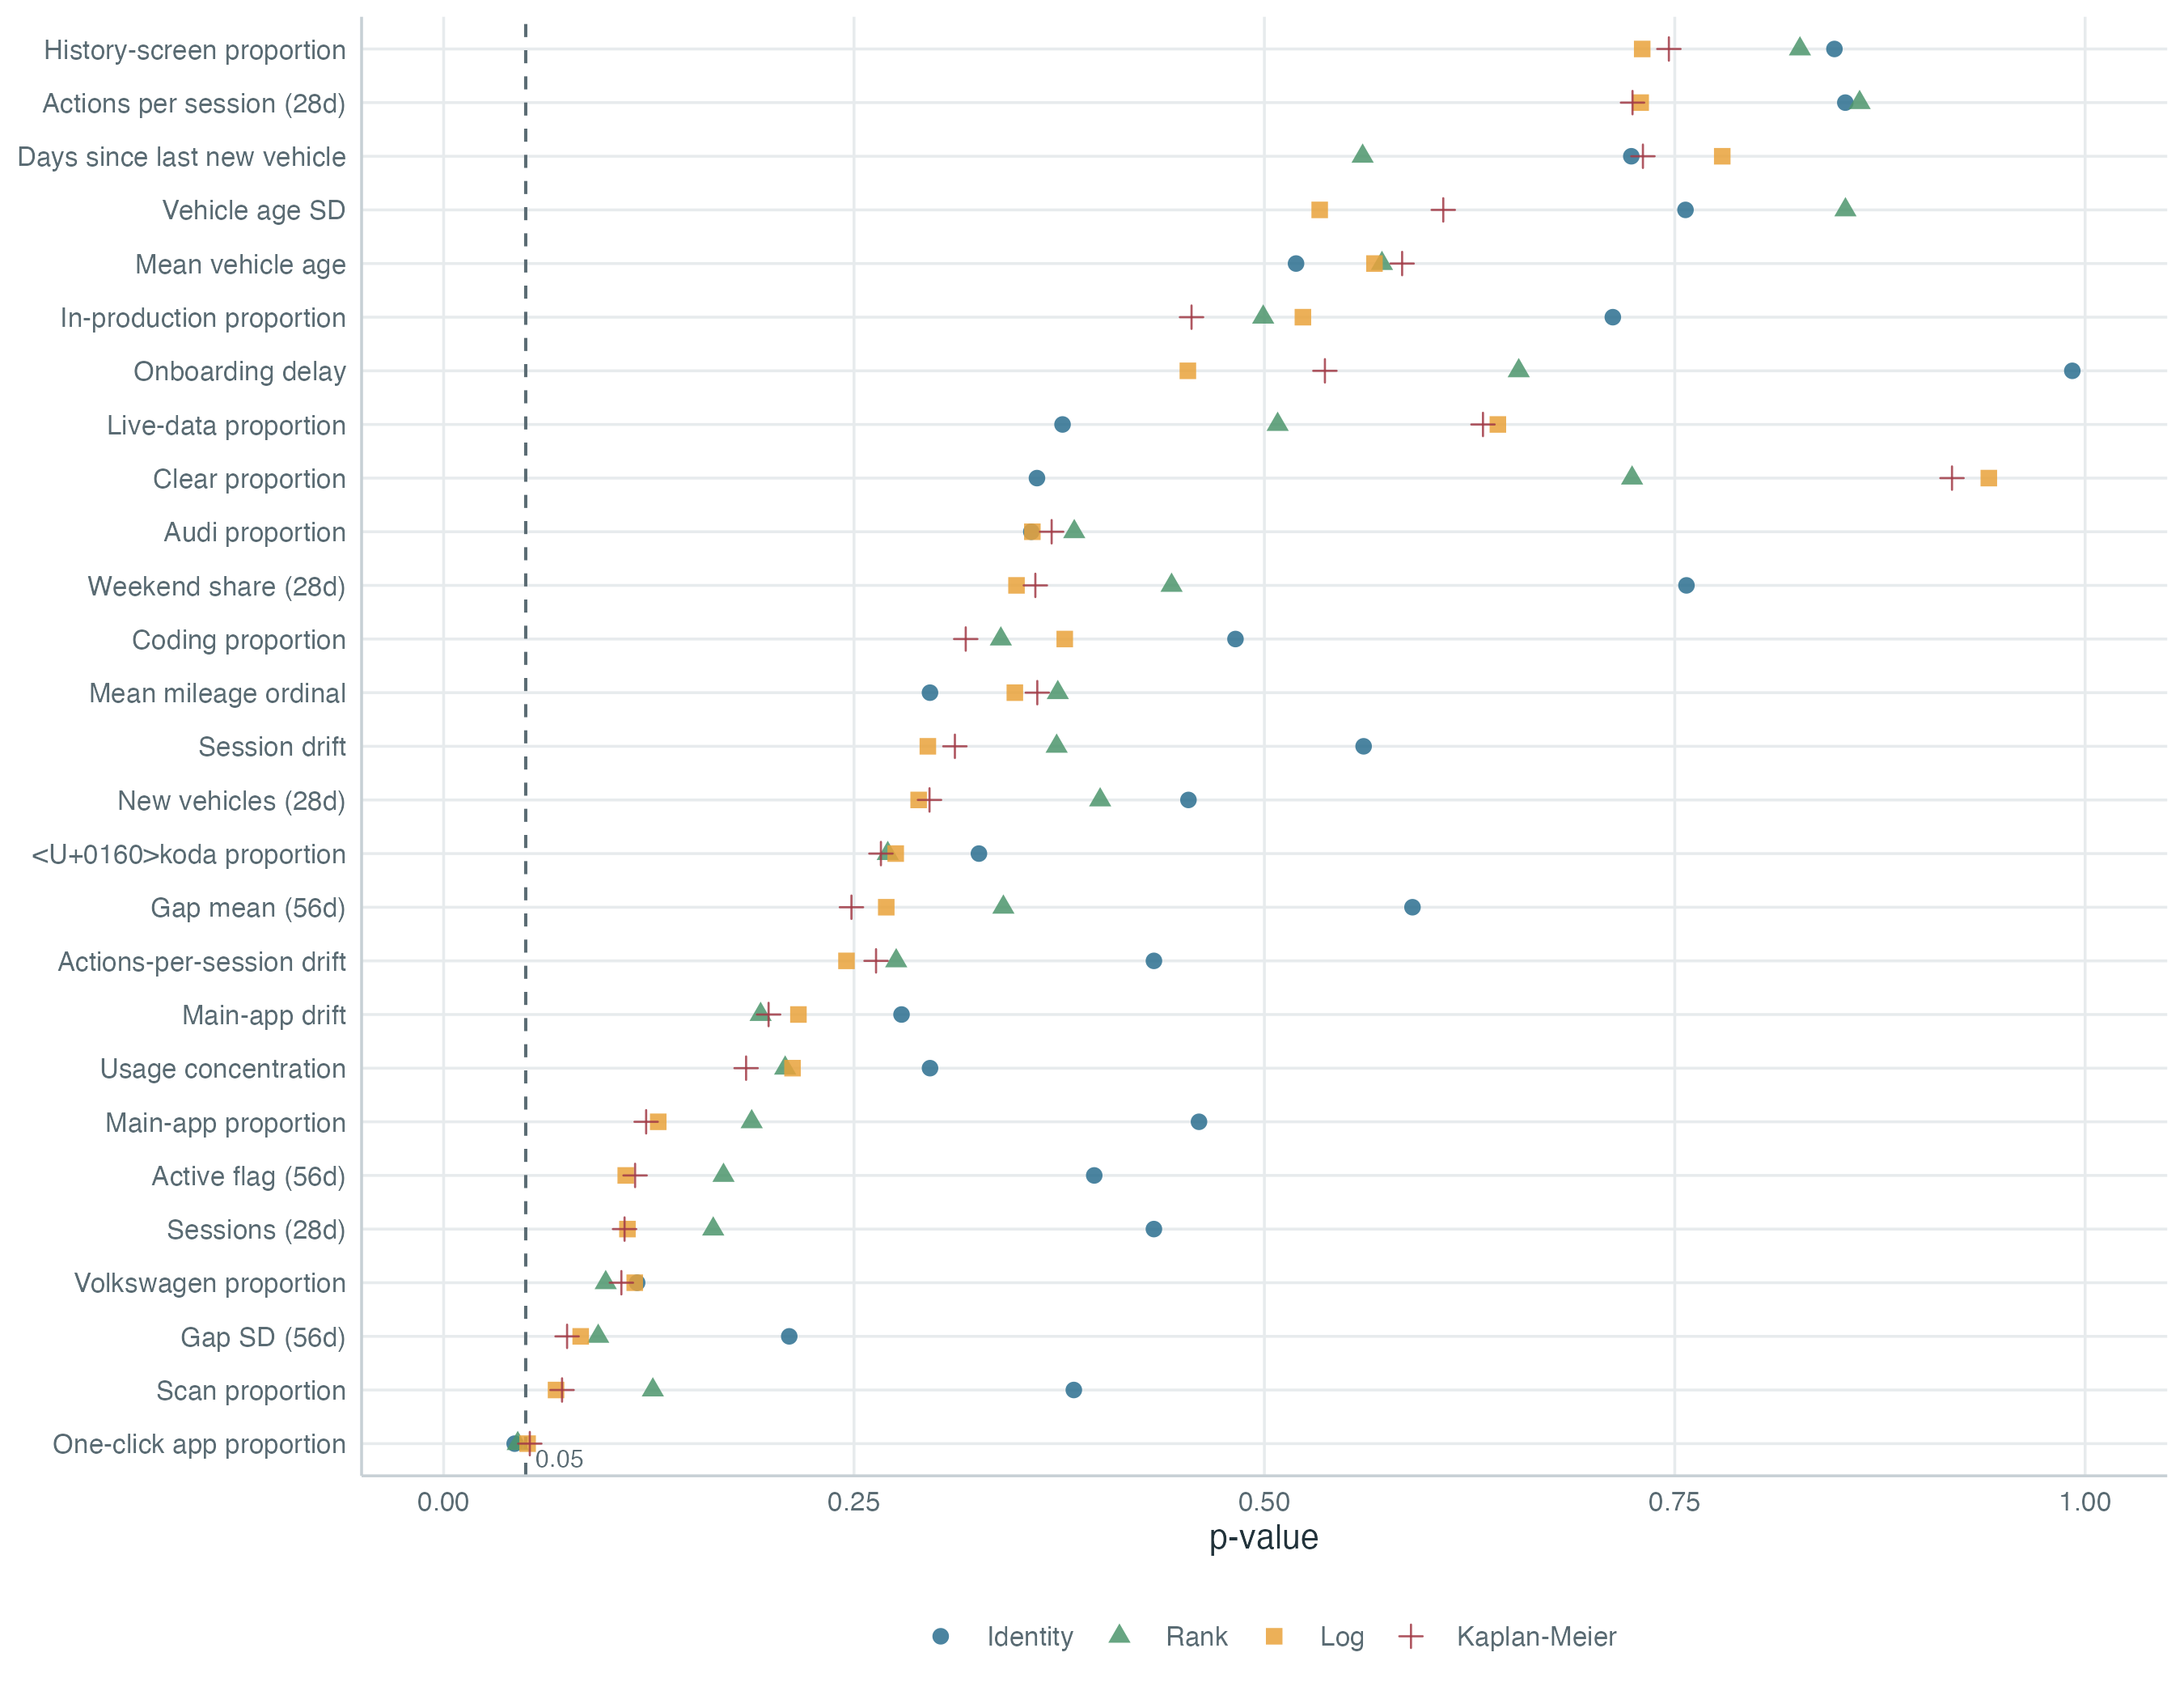
\includegraphics[width=\textwidth]{Images/09_ph_test_transforms.png}
\caption{Covariate-specific $p$-values under each transform. The dashed line is 0.05.}
\label{fig:ph-transforms}
\end{figure}
 
A null carries weight only if the test could have found a violation. \textcite{austin2018power} report that power stays low to moderate even at high event counts, which is reason enough to hold this result loosely. But the version used here also over-rejects when covariates are correlated, \textcite{metzger2024} find, and these covariates are (Section~\ref{sec:res-vif}). The test was if anything tilted toward finding the violation it did not find.
 
Neither consideration settles it, so M3 measures the departure instead of arguing about the test. Three covariates have a rank-transform $p$-value below 0.1, and M3 refits M0 with a time-transform term on each. A constant $\beta_k$ becomes $\beta_k(t) = \beta_k + \beta_k^{\text{tt}}\,g(t)$. What M3 reports is how far that coefficient travels between the first event time and the last. None of it is a hypothesis test, since they were chosen on M0's own results.
 
\begin{table}[htbp]
\centering
\small
\begin{tabular}{@{}lrrrrr@{}}
\toprule
Covariate & $\hat\beta$ (M0) & $\hat\beta^{\text{tt}}$ & $p$ & $\Delta\log$HR & HR start $\to$ end \\
\midrule
\multicolumn{6}{@{}l}{\emph{Identity transform, $g(t) = t$}} \\
One-click app proportion & $-0.4374$ & $+1.62\times10^{-3}$ & 0.038 & $+1.477$ & $0.65 \to 2.83$ \\
Volkswagen proportion    & $-0.0539$ & $-5.99\times10^{-4}$ & 0.119 & $-0.545$ & $0.95 \to 0.55$ \\
Gap SD (56d)             & $-0.0098$ & $-4.36\times10^{-5}$ & 0.223 & $-0.040$ & $0.99 \to 0.95$ \\
\addlinespace
\multicolumn{6}{@{}l}{\emph{Log transform, $g(t) = \log t$}} \\
One-click app proportion & $-0.4374$ & $+0.329$   & 0.048 & $+0.937$ & $0.65 \to 1.65$ \\
Volkswagen proportion    & $-0.0539$ & $-0.118$   & 0.116 & $-0.337$ & $0.95 \to 0.68$ \\
Gap SD (56d)             & $-0.0098$ & $-0.0114$  & 0.081 & $-0.033$ & $0.99 \to 0.96$ \\
\bottomrule
\end{tabular}
\caption{M3, fitted on the three covariates whose rank-transform \texttt{cox.zph} $p$-value falls below 0.1. $\Delta\log$HR is how far the log hazard ratio moves across the observed follow-up, and the last column gives the hazard ratio per unit at the first and last event time. The $p$-values are shown for completeness and are not valid tests, since the covariates were selected from M0.}
\label{tab:m3-drift}
\end{table}
 
The Volkswagen proportion travels $-0.55$ on the log scale over the whole of follow-up and gap SD travels $-0.04$, small enough that both hazard ratios stay on the same side of 1 throughout. Those two are stable in the sense the assumption requires. The one-click app proportion is not. Its coefficient travels $+1.48$, and the hazard ratio per unit runs from 0.65 at the first event time to 2.83 at the last, crossing 1 on the way. Early in follow-up it marks a customer as safer, late in follow-up it marks them as at risk, and one number cannot say both. The log transform gives the same picture at a smaller magnitude, so the finding is not an artefact of the time scale.
 
Those endpoint ratios are per unit, and a unit is the whole range of a proportion whose standard deviation is 0.18. Almost no customer moves that far, so the per-unit figures describe a change the data do not contain. Rescaled to one standard deviation, the same drift runs from a hazard ratio of 0.924 at the first event time to 1.206 at the last.
% TODO VERIFY: 0.924 and 1.206 computed as exp(-0.4374*0.17995) and
% exp((-0.4374 + 1.477)*0.17995), using sd_x = 0.17995 from coefficients_m0.csv.
% The 0.924 matches tab:coefficients, which is the check. Recompute from the
% fitted object before this goes in. Log transform gives 0.924 -> 1.094.
The scale of the departure shrinks by an order of magnitude under that rescaling. The sign reversal does not. A covariate whose hazard ratio crosses 1 partway through follow-up is doing something a single coefficient cannot represent, however modest the distance travelled.
 
How much weight that carries is limited. It is one covariate of twenty-seven, and it was selected on its own $p$-value, which is not a basis for inference. That $p$-value also straddles 0.05, reaching significance under two transforms and not the other two. Against both, its M0 coefficient is significant at $p = 0.0002$, so this is not a covariate the model is otherwise ignoring.
 
% ============================================================
% RQ1 VERDICT --- WRITE ONE OF THESE, DELETE THE OTHER.
% Both are drafted to follow the paragraph above without any
% restructuring. Neither is a commitment until you pick.
%
% ----- VERSION A: the assumption holds, exception is a footnote -----
% Taken together these favour reading the flag as chance. The global
% test does not reject on any transform, the one covariate that
% crosses 0.05 does not do so consistently, and the departure it
% shows is modest once expressed on a scale customers actually move
% across. Proportional hazards is treated as holding for this frame,
% and the one-click app proportion is noted as the covariate to watch
% should the model be refitted on a longer window.
%
% ----- VERSION B: holds globally, one documented exception -----
% Taken together these place the finding between the two readings the
% test alone offers. Proportional hazards holds for the frame as a
% whole, and no aggregate diagnostic would have said otherwise. One
% covariate nonetheless carries an effect that reverses direction over
% follow-up, and that is a fact about the model a practitioner
% deploying it would need. The value of testing the assumption rather
% than asserting it lies exactly there, since the global result and
% the assertion it replaces agree, while only the test identifies
% which covariate the agreement conceals.
% ============================================================
 
\subsection{Assumption 2: do the covariates enter as straight lines?}
\label{subsec:res-linearity}
 
Proportional hazards survives, so the second assumption can be tested inside models that impose the first. M1 and M2b replace $\beta_k x_k$ with a restricted cubic spline for each continuous covariate, using \texttt{splines::ns} with three degrees of freedom. That places two interior knots at the 33rd and 67th percentiles and holds the fitted curve linear beyond the outer knots, so each splined covariate carries three parameters instead of one.
 
Not every covariate can take a spline. Two interior knots collapsing onto the minimum leaves the basis rank deficient, which happens for a proportion that is zero on most rows. Eighteen of the twenty-seven pass that check in every training fold and are splined. The remaining nine stay linear in all four models, and Table~\ref{tab:coefficients} marks which is which. The likelihood ratio test therefore carries $18 \times 2 = 36$ degrees of freedom.
 
The statistic is twice the difference in maximised log-likelihood,
%
\begin{equation}
\chi^2_{\text{LR}} = 2\big(\ell_{\text{spline}} - \ell_{\text{linear}}\big) \sim \chi^2_{q},
\label{eq:lr-statistic}
\end{equation}
%
with $q$ the number of additional parameters \parencite{wilks1938}. The linear model is nested inside the spline model, since setting the two non-linear basis coefficients of each covariate to zero recovers it. That nesting is what makes the test valid.
 
The same test is run twice, once under each link (Figure~\ref{fig:linearity-grid}).
 
\begin{table}[htbp]
\centering
\small
\begin{tabular}{@{}llrrr@{}}
\toprule
Comparison & Link & $\chi^2$ & df & $p$ \\
\midrule
M0 against M1   & Cox                   & 109.85 & 36 & $2.1\times10^{-9}$ \\
M2a against M2b & Complementary log-log & 111.61 & 36 & $1.1\times10^{-9}$ \\
\bottomrule
\end{tabular}
\caption{Likelihood ratio tests of the linear specification against restricted cubic splines. The 5\% critical value of $\chi^2_{36}$ is 51.0.}
\label{tab:lrt}
\end{table}
 
Linearity is rejected under both links, and the two statistics are within two units of each other. Both sit at roughly twice the 5\% critical value, so this is not a borderline result.
 
One route to that rejection has nothing to do with curvature. Efron's approximation could account for it, and event times falling on interval boundaries with the tie structure of Section~\ref{sec:res-ties} is exactly the situation where it might. M0 and M2a estimate the same $\beta$ by \eqref{eq:cloglog}, differing only in whether the ties are approximated, so any gap between them belongs to Efron.
 
\begin{table}[htbp]
\centering
\small
\begin{tabular}{@{}lr@{}}
\toprule
Quantity & Value \\
\midrule
Correlation between coefficient vectors & 0.99999 \\
Mean absolute relative difference & 2.0\% \\
Largest absolute difference & $4.4\times10^{-3}$ \\
Largest relative difference, all 27 & 13.8\% \\
\bottomrule
\end{tabular}
\caption{Agreement between M0 and M2a. The 13.8\% figure is on days since last new vehicle, whose coefficient is $-2.3\times10^{-4}$, so the relative difference there carries no information.}
\label{tab:tie-agreement}
\end{table}
 
The coefficient vectors correlate at 0.99999 and the mean absolute relative difference is 2.0\%. Efron is not moving these estimates.
 
\begin{figure}[htbp]\centering
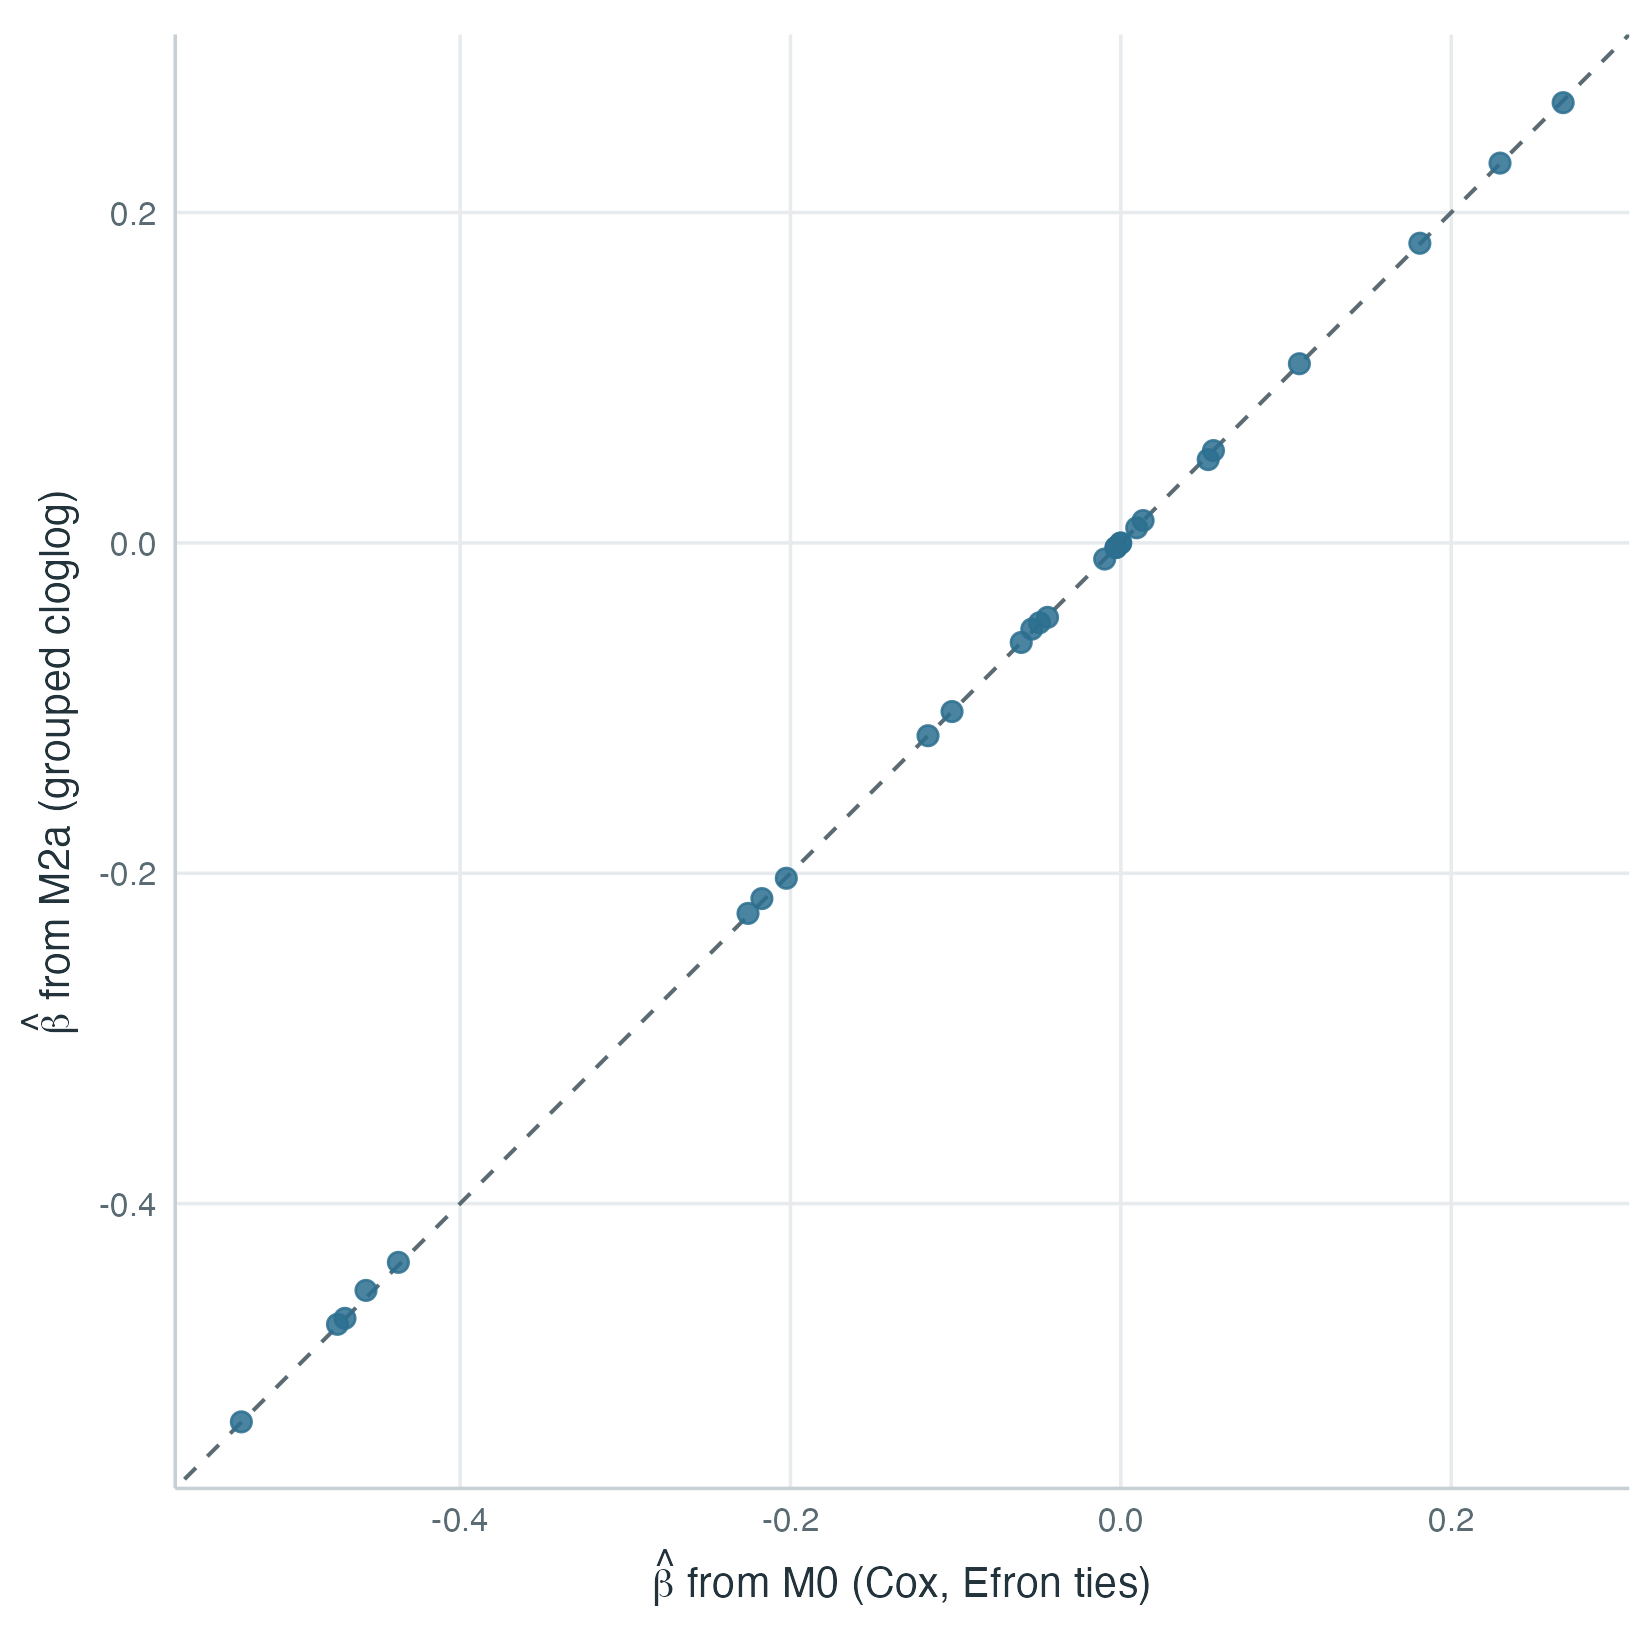
\includegraphics[width=0.6\textwidth]{Images/11_tie_agreement.png}
\caption{M0 against M2a coefficients. Points on the diagonal mean the tie approximation costs nothing.}
\label{fig:tie-agreement}
\end{figure}
 
Out of fold they are indistinguishable too, at 0.6803 against 0.6804 in mean AUC and with a Brier difference below $10^{-6}$ (Table~\ref{tab:cv-paired}). The rejection is about the functional form, not about how the estimator handles ties.
 
% ============================================================
% RQ1 VERDICT, BOTH ASSUMPTIONS TOGETHER.
% The factual setup is written below. What is missing is the sentence
% that says what the combination means for the Section 2.4 critique.
% Points available to you, all established above.
%   - PH not rejected on any of four transforms, with the one flagged
%     covariate consistent with chance at 27 tests.
%   - Linearity rejected at p < 1e-8 under both links, at twice the
%     critical value, and not attributable to Efron.
%   - The applied literature asserts both and tests neither.
% ============================================================
The two assumptions therefore come apart. One survives every test the design can bring against it, and the other fails both, decisively and under two independent links. The applied papers of Chapter~2 assert the pair together, as a single condition for using the model at all.
% TODO replace "Chapter~2" with \ref{} to your applied-literature section.
 
% [YOUR SENTENCE HERE: what it means that one assertion survives and
%  the other does not. This is the RQ1 answer.]
 
\subsection{What relaxing the assumptions buys}
\label{subsec:res-oof}
 
Rejecting linearity is a statement about the data the models were fitted on. Whether the curvature carries to customers no model has seen is a separate question, and it is the one RQ2 asks. The protocol is that of Figure~\ref{fig:cv-protocol}. M4 enters here and only here, imposing neither assumption.
 
% ============================================================
% MOVE THIS TO METHOD, Section~\ref{subsec:validation}. It states how a
% predicted hazard is formed, which is a criterion, not a result. Left
% here so you can cut and paste it, then replace with a forward ref.
%
% Turning a Cox fit into a probability for one interval requires the
% baseline hazard back, since the partial likelihood cancelled it during
% estimation. The predicted hazard on the window $(t_1, t_2]$ is
% $1 - \exp(-\Delta\hat\Lambda_0 \exp(x'\hat\beta))$, with
% $\Delta\hat\Lambda_0 = \hat\Lambda_0(t_2) - \hat\Lambda_0(t_1)$ read off
% the Breslow estimator. Because that estimator only steps at observed
% event times, $\hat\Lambda_0$ is set to zero before the first of them
% rather than extrapolated backwards. M2a and M2b need no such step,
% carrying a free intercept per interval instead, which is why the two
% families can be compared on the same rows at all.
% ============================================================
How a fitted model becomes a predicted probability for one interval is set out in Section~\ref{subsec:validation}, and it differs between the two families in a way that matters for reading the table below.
 
\begin{table}[htbp]
\centering
\small
\begin{tabular}{@{}lrrr@{}}
\toprule
Model & AUC & Brier & Calibration slope \\
\midrule
M0  & 0.6803 (0.0102) & 0.021536 (0.000156) & 0.919 (0.080) \\
M1  & 0.6822 (0.0099) & 0.021534 (0.000152) & 0.893 (0.080) \\
M2a & 0.6804 (0.0108) & 0.021536 (0.000156) & 0.934 (0.081) \\
M2b & 0.6826 (0.0106) & 0.021533 (0.000152) & 0.907 (0.079) \\
M4  & 0.6856 (0.0121) & 0.021517 (0.000156) & 0.981 (0.092) \\
\bottomrule
\end{tabular}
\caption{Out-of-fold performance, mean across five folds with the standard deviation between folds in brackets. The base rate is 2.22\% of rows, so a model predicting that rate for every row scores a Brier of 0.02174.}
\label{tab:cv-metrics}
\end{table}
 
\begin{table}[htbp]
\centering
\small
\begin{tabular}{@{}lrrc@{}}
\toprule
Comparison & $\Delta$ AUC & $\Delta$ Brier & Folds improved \\
\midrule
M1 against M0   & $+0.0019$ & $-0.000002$ & 4 of 5 \\
M2b against M2a & $+0.0022$ & $-0.000003$ & 4 of 5 \\
M2a against M0  & $+0.0001$ & $\approx 0$ & 3 of 5 \\
M4 against M0   & $+0.0053$ & $-0.000020$ & 5 of 5 \\
M4 against M1   & $+0.0033$ & $-0.000017$ & 4 of 5 \\
\bottomrule
\end{tabular}
\caption{Paired fold-by-fold differences. The same folds are used throughout, so these are matched comparisons. A negative $\Delta$ Brier is an improvement.}
\label{tab:cv-paired}
\end{table}
 
\begin{figure}[htbp]\centering
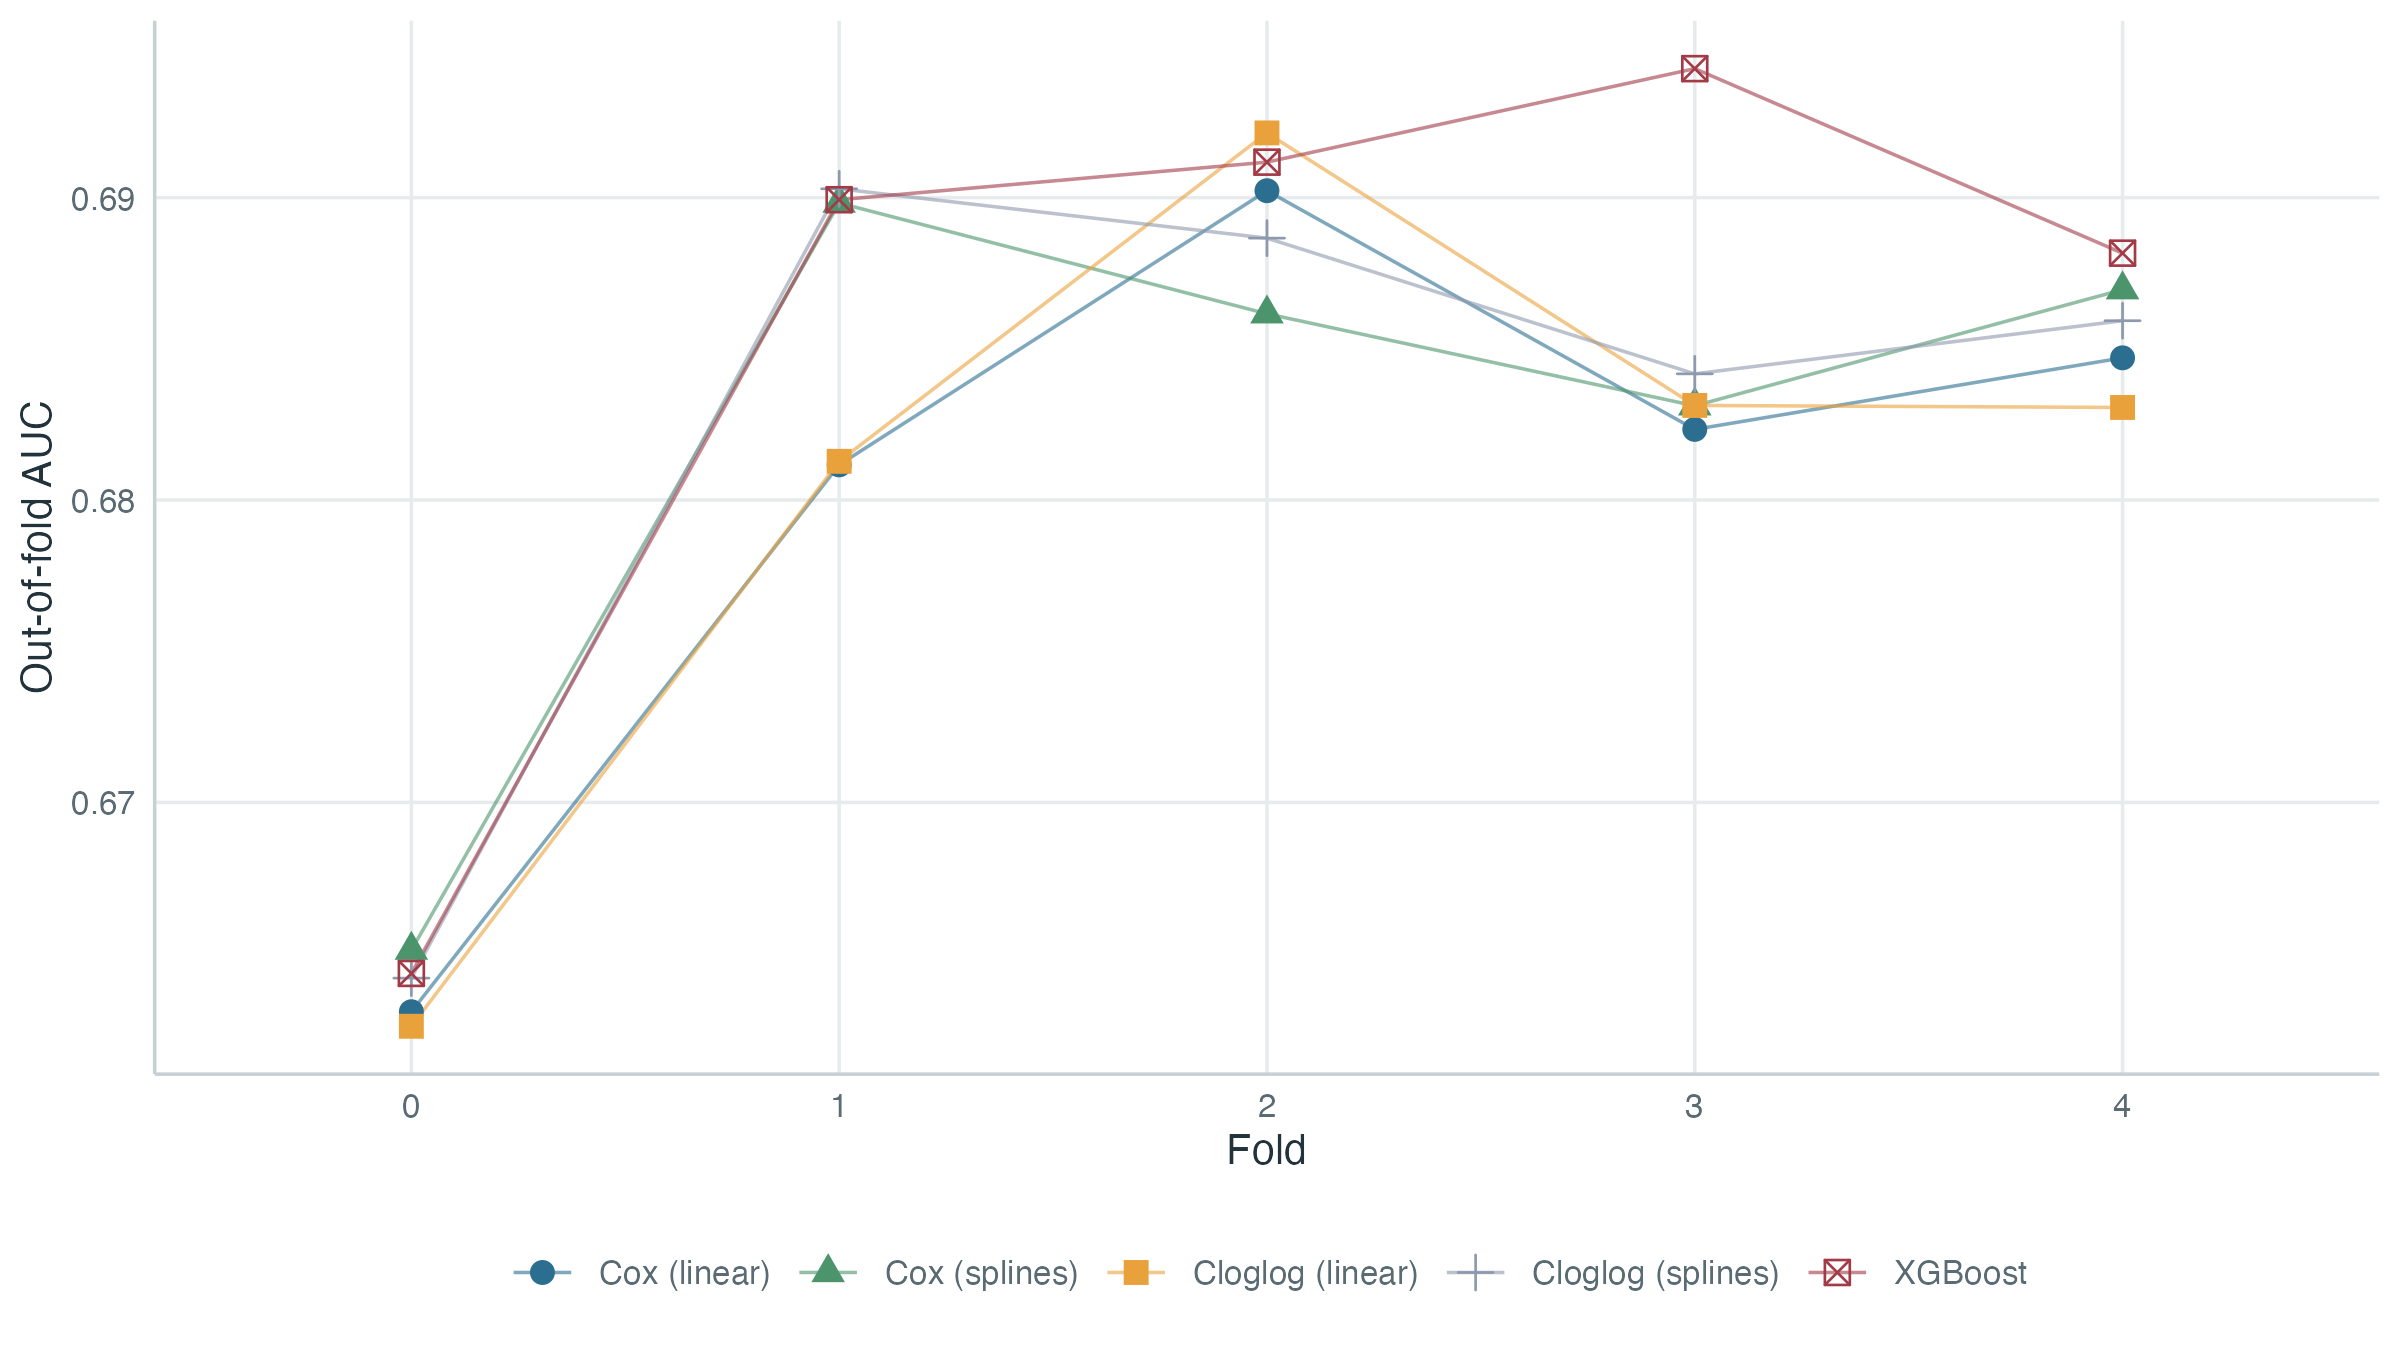
\includegraphics[width=\textwidth]{Images/13_auc_by_fold.png}
\caption{Out-of-fold AUC by fold. The spline models sit above the linear ones in four folds of five, and M4 sits above M0 in every fold and above M1 in four of five.}
\label{fig:auc-folds}
\end{figure}
 
Relaxing linearity gains 0.0019 AUC on average and improves four folds of five, against a fold-to-fold spread of 0.010. The direction holds across folds, but a gain of 0.0019 does not survive a spread of 0.010. Brier cannot separate them at all. Predicting 2.22\% for every row already scores 0.02174, so the twenty-seven covariates together buy 0.0002 of it, and one specification differs from another somewhere inside that margin. A departure from linearity that the likelihood ratio test rejects at $p < 10^{-8}$ is worth 0.0019 AUC to a customer the model has not seen.
 
M4's seven hyperparameters are tuned inside each outer fold on an inner five-fold split by log loss, and Table~\ref{tab:xgb-params} gives the winning setting per fold. No two folds converge on the same configuration: max depth is 3 in three folds and 4 in the other two, the learning rate is 0.05 in four folds and 0.03 in the fifth, and the boosting rounds range from 100 to 400.

\begin{table}[htbp]
\centering
\small
\begin{tabular}{@{}rrrrrrrr@{}}
\toprule
Fold & Max depth & Learning rate & Rounds & Min child weight & Row subsample & Column subsample & $L_2$ \\
\midrule
0 & 3 & 0.05 & 200 & 5 & 1.0 & 1.0 & 5 \\
1 & 4 & 0.03 & 400 & 1 & 0.6 & 0.6 & 10 \\
2 & 3 & 0.05 & 200 & 5 & 0.6 & 0.6 & 10 \\
3 & 4 & 0.05 & 200 & 3 & 0.8 & 0.6 & 5 \\
4 & 3 & 0.05 & 100 & 1 & 0.6 & 1.0 & 1 \\
\bottomrule
\end{tabular}
\caption{Winning XGBoost hyperparameters per outer fold, selected on mean inner-fold log loss.}
\label{tab:xgb-params}
\end{table}

Relaxing both assumptions at once now pays off. M4 gains 0.0053 AUC against M0, in five folds of five, and 0.0033 against M1, in four of five, with Brier moving in its favour by about $2\times10^{-5}$ either way. Calibration is the measure it wins most clearly, at a slope of 0.981 where the Cox family sits between 0.89 and 0.93, and no other model in the study comes that close to the ideal of 1. M4 now leads the ladder on discrimination and calibration together, not on one at the other's expense.
 
\begin{figure}[htbp]\centering
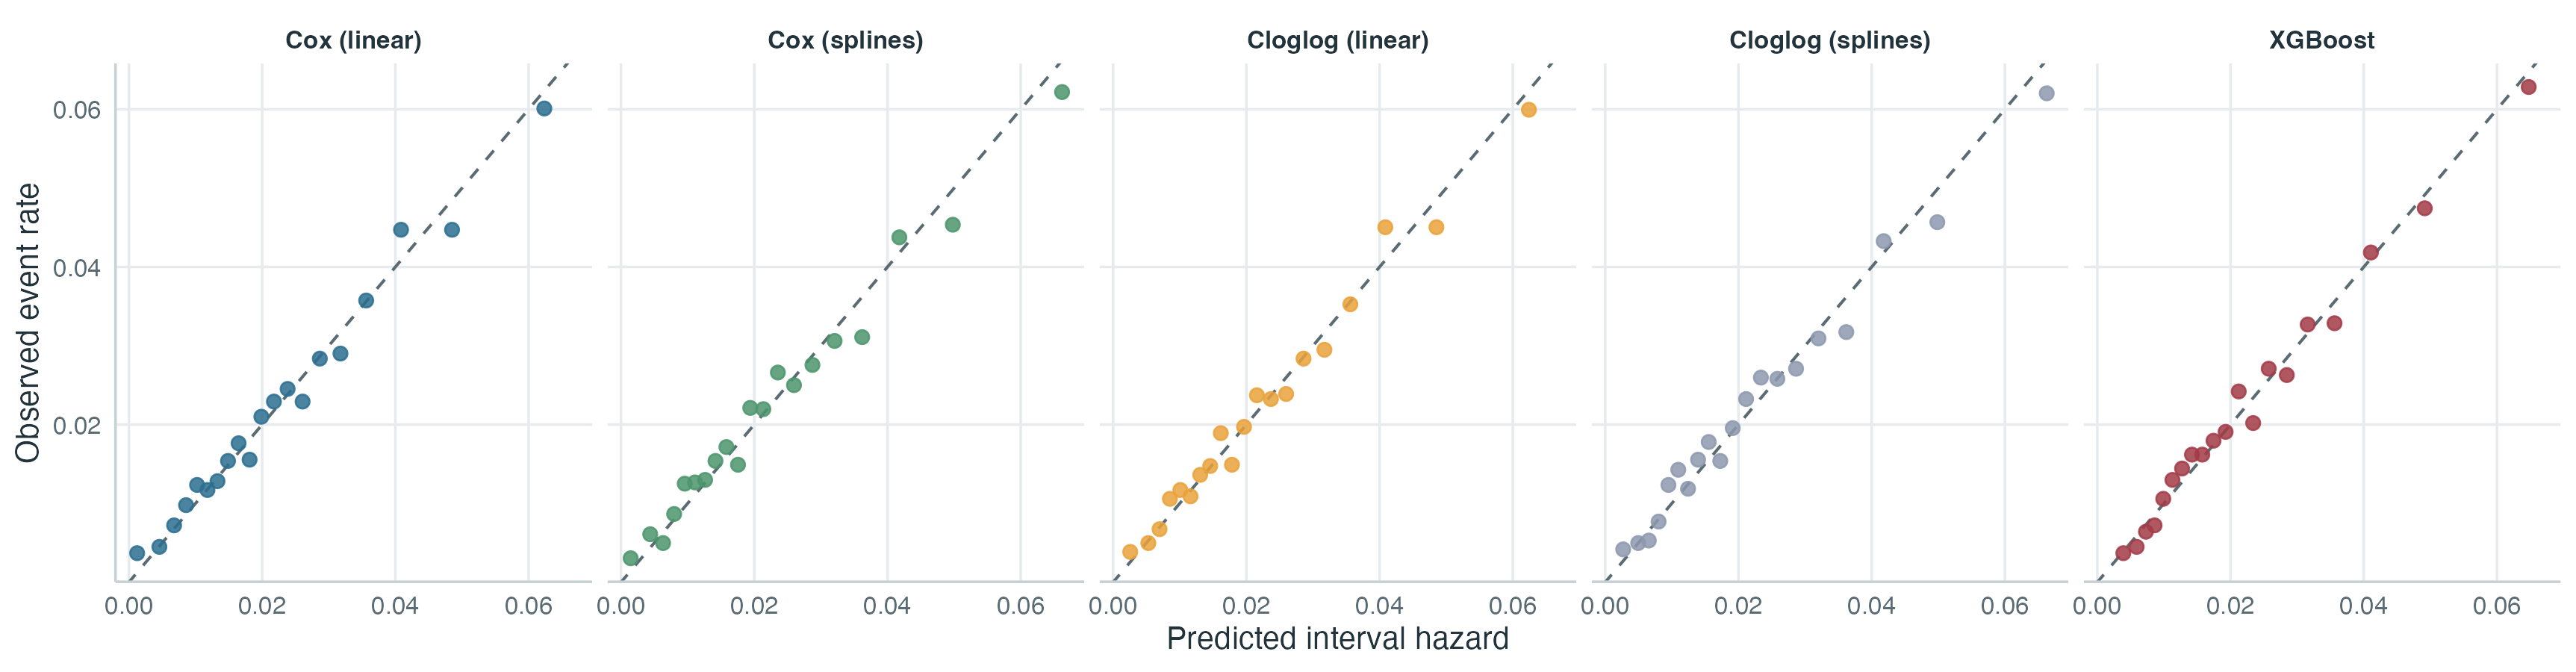
\includegraphics[width=\textwidth]{Images/12_calibration.png}
\caption{Predicted against observed, by twentieth of the predicted hazard. The Cox family sits below the diagonal at the top end, which is the overconfidence that the calibration slopes in Table~\ref{tab:cv-metrics} record. M4 does not.}
\label{fig:calibration}
\end{figure}
 
% ============================================================
% TODO --- INTERVAL-WIDTH SENSITIVITY CHECK HAS NO DATA.
% metrics_summary_m2b_28day.csv and metrics_sensitivity_m2b_14_vs_28.csv
% were both overwritten on the last run with a 14-day five-model
% comparison carrying the pre-fix Cox numbers, and
% oof_predictions_m2b_28day.csv holds 124,783 rows x 5 models, which is
% the 14-day frame, not the 28-day one. Re-run
% Coding/R/sensitivity_m2b_28day.R, then restore the paragraph and
% tab:sensitivity-width here. Until then this subsection makes no
% claim about the interval width.
% ============================================================
 
One qualification bounds what that lead can claim. Like M2a and M2b, M4 needs a stand-in for the baseline hazard that the partial likelihood cancels out of M0 and M1, and it gets one: the interval index enters as a covariate in its own right, the discrete-time counterpart of $\Lambda_0(t)$. Withholding it would have left M4 the only model in the ladder denied a baseline, confounding any gap with the two assumptions RQ1 asks about rather than isolating them. What that covariate carries, though, is selection as much as time: a customer still at risk late in follow-up is one with lower unobserved frailty by construction, and a tree fits that selection as readily as it fits a genuine covariate effect. That is admissible for ranking customers out of fold, which is what Table~\ref{tab:cv-metrics} scores, and it is not evidence about what causes churn.
 
% ============================================================
% RQ2 VERDICT. The mechanisms are set out below as candidates, which
% is as far as the evidence here goes on its own. What is missing is
% which one the thesis backs and on what grounds.
% ============================================================
Two different questions sit behind these numbers, and the data separate them only partly. Why splines add so little within the Cox family is one: the covariates were built as proportions, rates and drifts rather than raw counts, so much of the curvature a flexible learner would have to discover is already encoded in how they are measured. Why M4 now gains is the other, and Section~\ref{subsec:res-shap} points to where: the interval index, standing in for M4's baseline, carries more weight in its predictions than any of the twenty-seven covariates the two families share. None of the Cox-family models let time interact with a covariate -- M3 fits that interaction for three of them by hand, and the rest of the ladder does not fit it at all -- while a tree searches for such interactions freely, which would explain a real gain the splines never touched. It would fit the selection reading above just as well: a covariate correlated with how long a customer survives to be observed gains exactly this kind of leverage without describing anything causal. The two readings are not distinguished here.
 
% [YOUR PARAGRAPH HERE: which reading the thesis takes and why. This
%  is the answer to RQ2. Note that the three mechanisms are not
%  mutually exclusive, and that the first explains the small spline
%  gain while the second explains why M4 loses in five folds of five
%  rather than in three or four.]
 
\subsection{What the flexible model uses instead}
\label{subsec:res-shap}
 
M4 is free of both assumptions and now discriminates better than every other model in the ladder, which makes it worth asking what it leans on to get there. SHAP attributes each prediction to the covariates that produced it \parencite{lundberg2017}, and the values here are computed out of fold, each row scored only by the fold model that never trained on it, so the ranking carries no leakage.
 
\begin{figure}[htbp]\centering
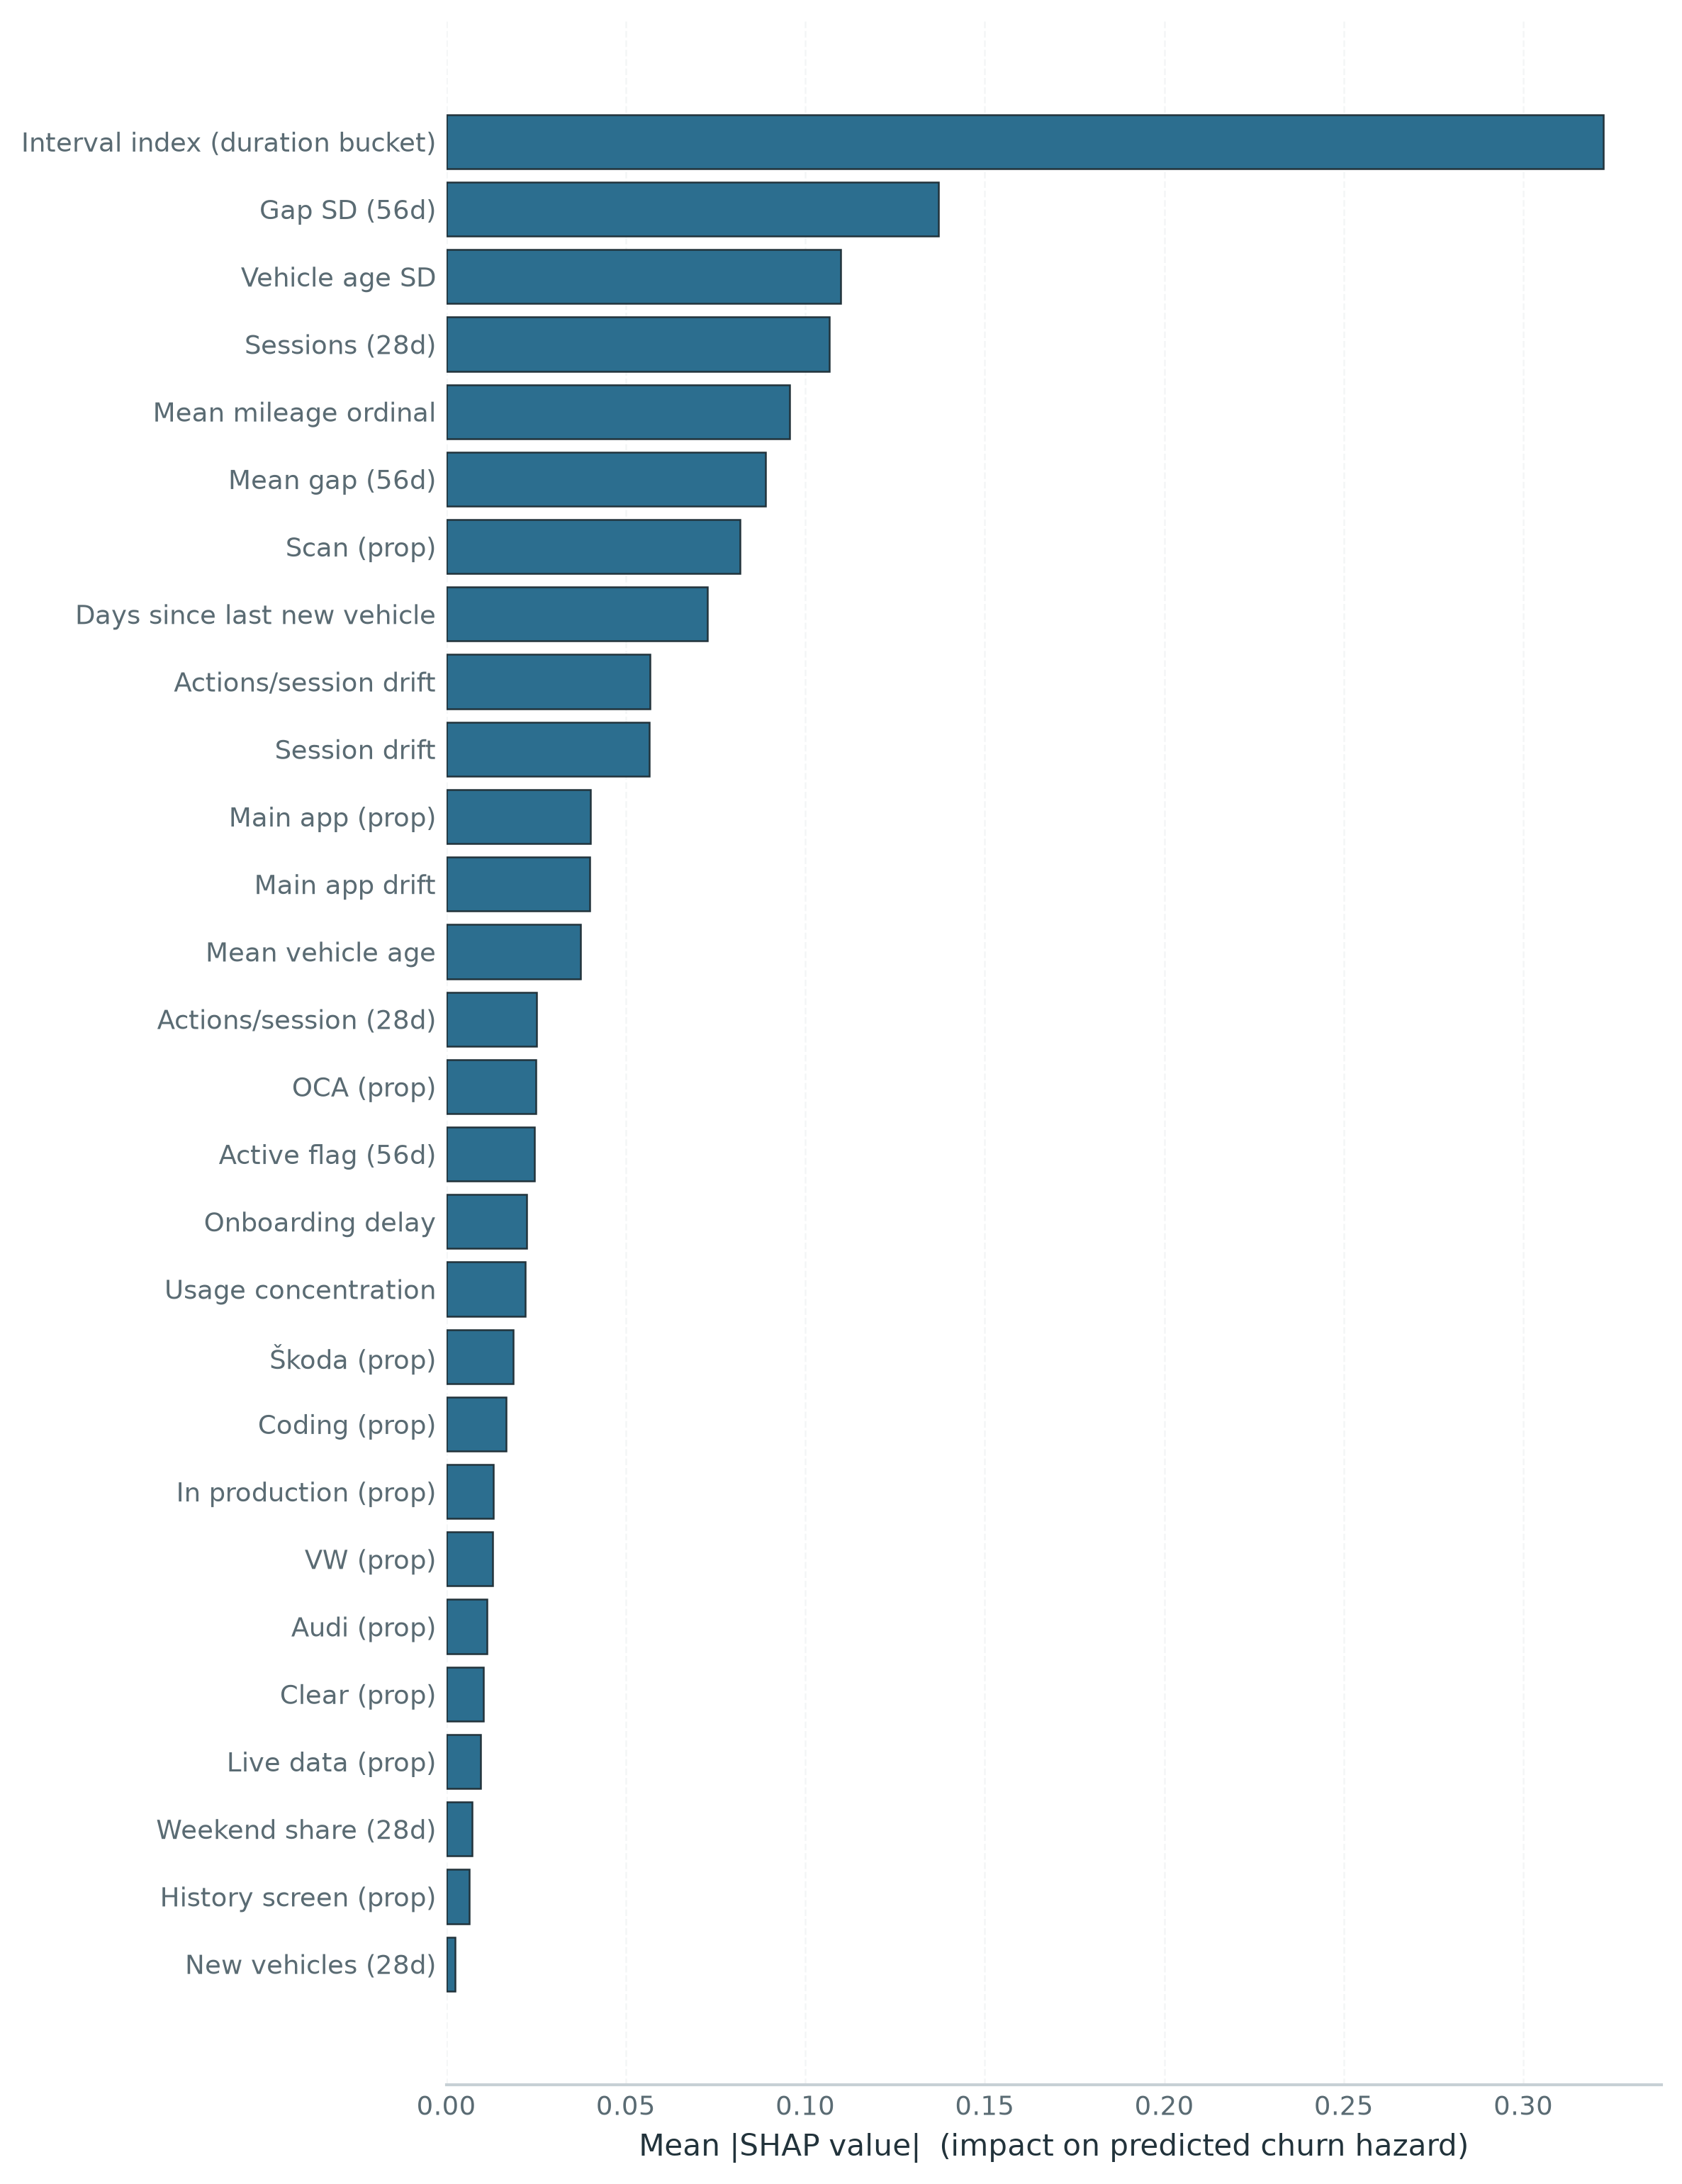
\includegraphics[width=0.85\textwidth]{Images/16_shap_importance.png}
\caption{Mean absolute SHAP value per covariate, out of fold. The ordering is by average contribution to the predicted hazard and carries no sign.}
\label{fig:shap-importance}
\end{figure}
 
\begin{figure}[htbp]\centering
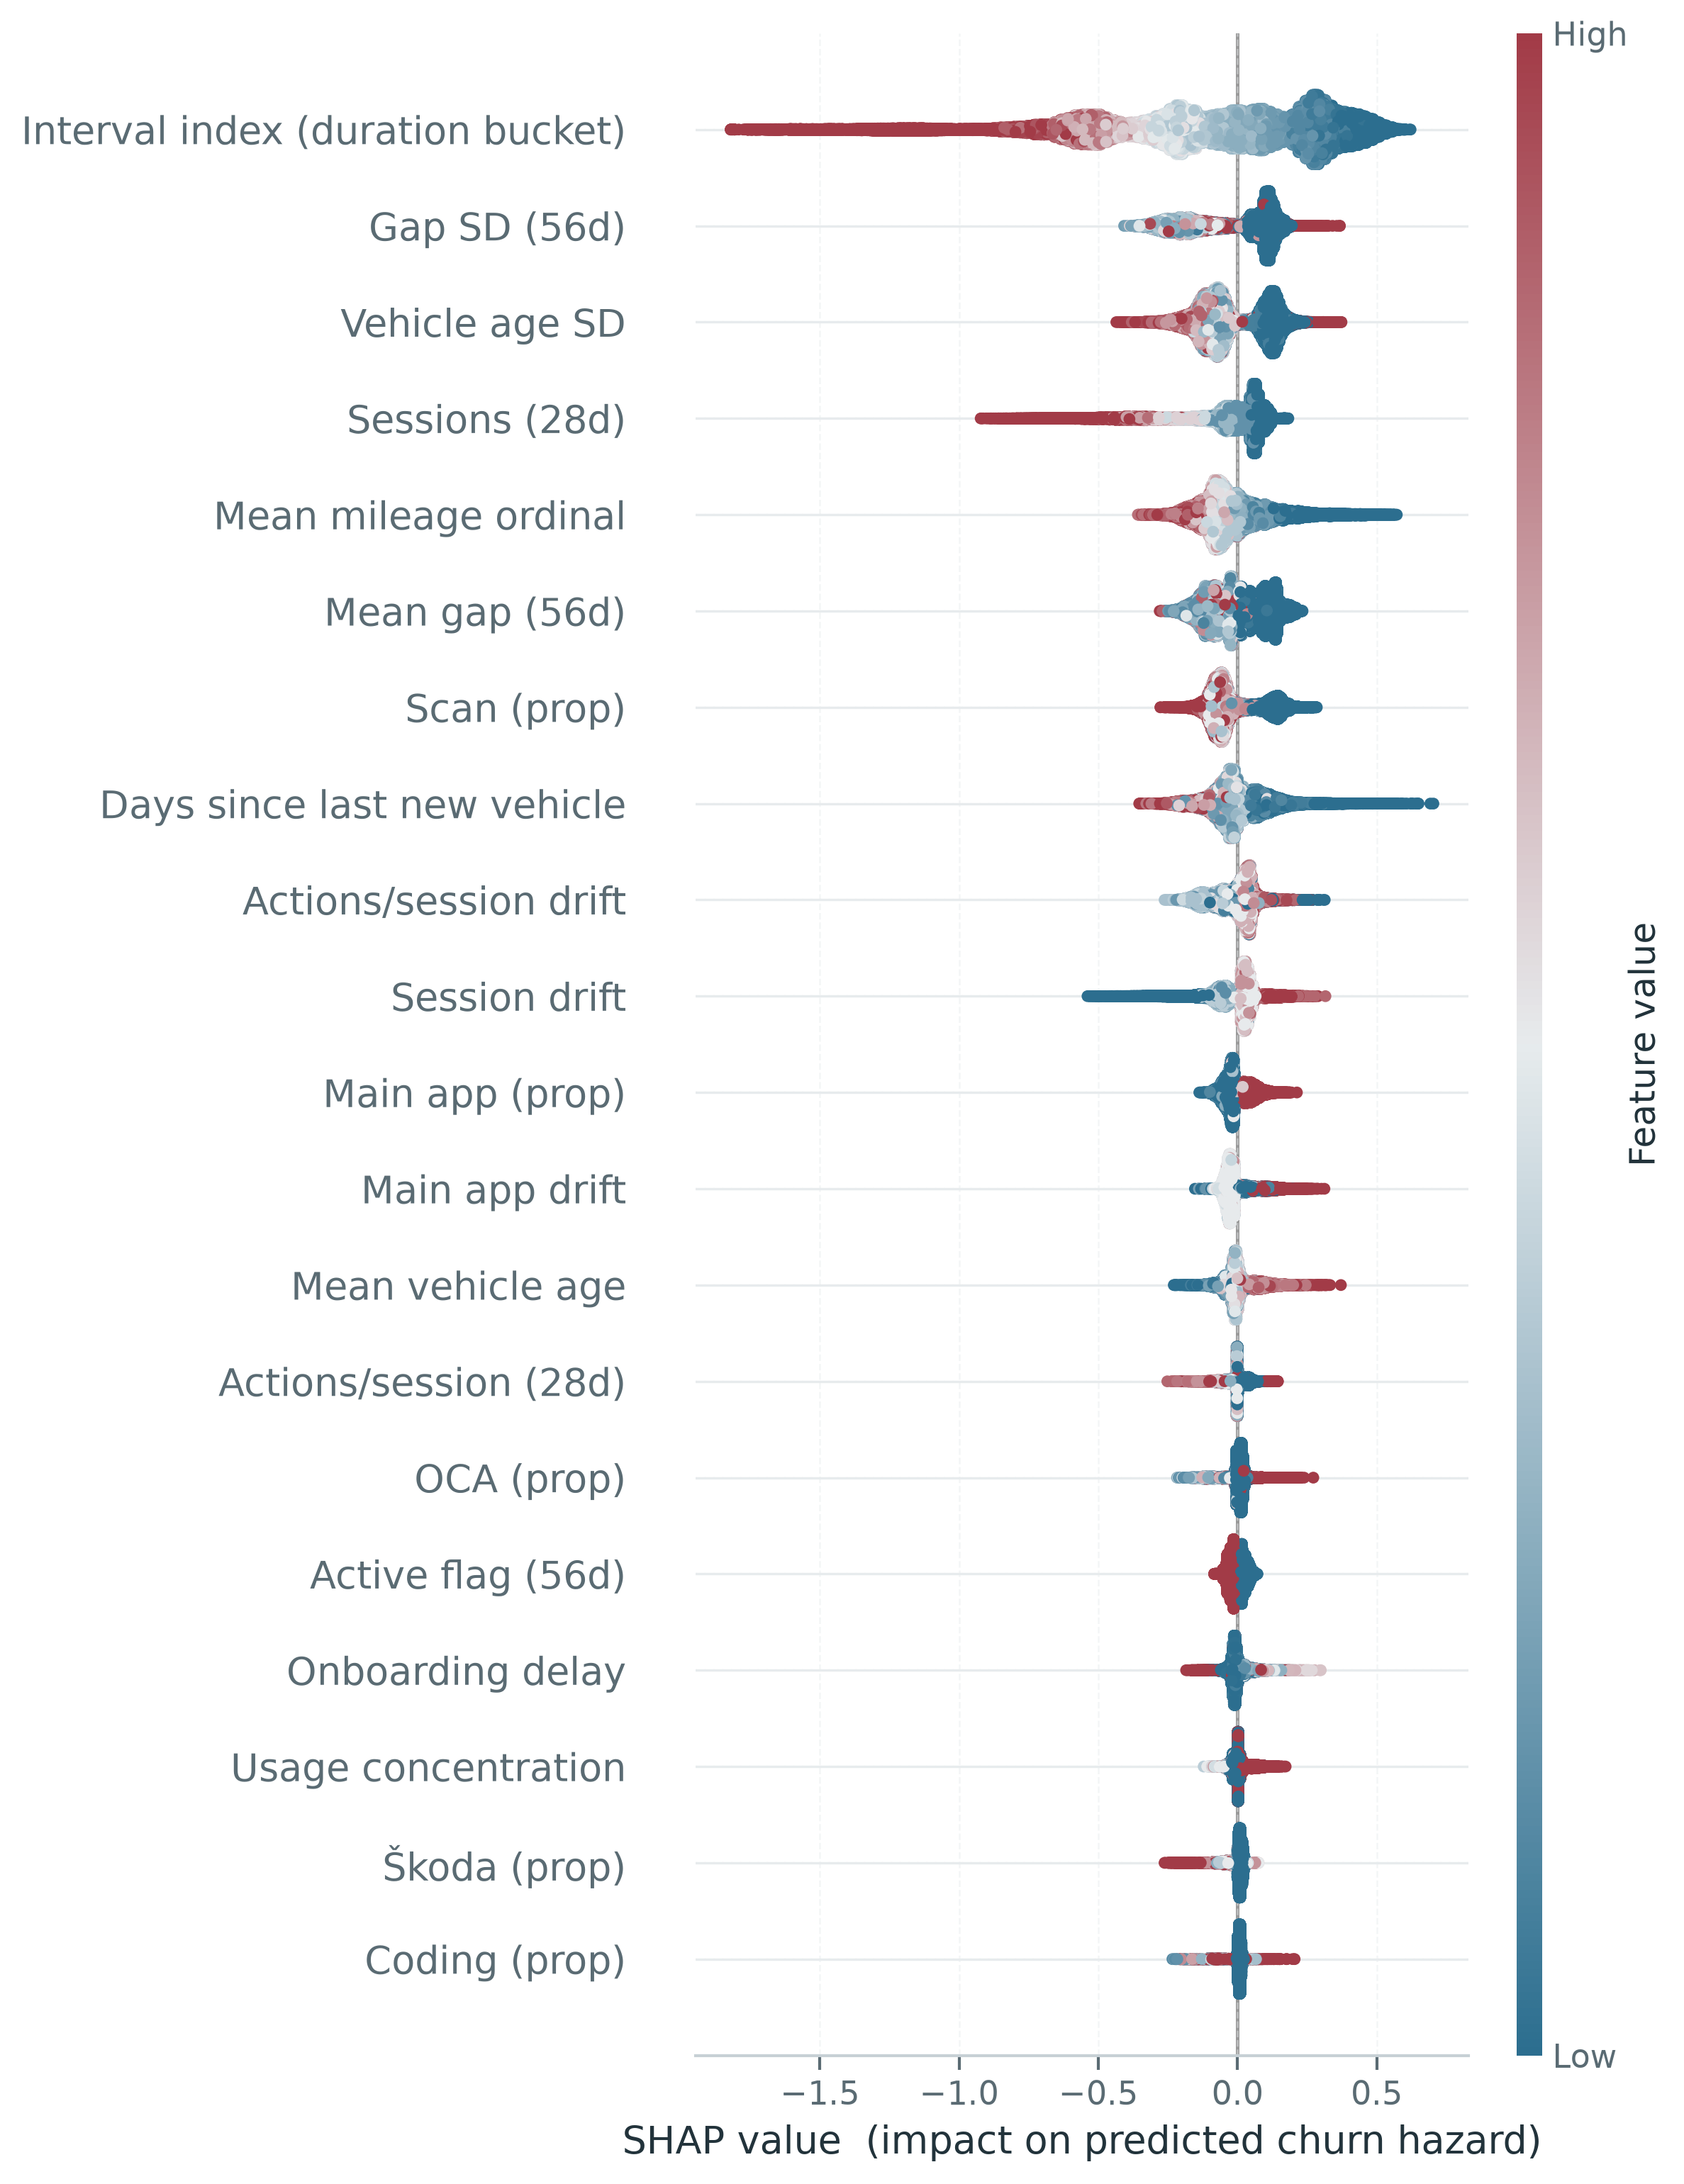
\includegraphics[width=0.85\textwidth]{Images/17_shap_summary.png}
\caption{Out-of-fold SHAP values by covariate. Horizontal position is the pull on the predicted hazard for one row, colour is that row's own value of the covariate. A block of high values to the right of zero means large values of the covariate raise the hazard.}
\label{fig:shap-summary}
\end{figure}
 
One covariate dwarfs every other in that ranking. The interval index -- the duration bucket standing in for M4's baseline (Section~\ref{subsec:res-oof}) -- carries a mean $|$SHAP$|$ of 0.322, more than double the next covariate and about a fifth of everything the model attributes across all twenty-eight inputs. It has no counterpart in M0, which recovers the same baseline as $\Lambda_0(t)$ rather than as a covariate with a coefficient, so it sits outside the comparison below. Table~\ref{tab:shap-vs-m0} gives the ten covariates M4 relies on most among the twenty-seven it shares with M0.

\begin{table}[htbp]
\centering
\small
\begin{tabular}{@{}lrrr@{}}
\toprule
Covariate & Mean $|$SHAP$|$ & M0 rank by $|z|$ & M0 $p$ \\
\midrule
Gap SD (56d)                 & 0.137 & 15 & 0.065 \\
Vehicle age SD               & 0.110 & 6  & $<0.001$ \\
Sessions (28d)               & 0.107 & 1  & $<0.001$ \\
Mean mileage ordinal         & 0.096 & 5  & $<0.001$ \\
Mean gap (56d)               & 0.089 & 22 & 0.430 \\
Scan proportion              & 0.082 & 2  & $<0.001$ \\
Days since last new vehicle  & 0.073 & 21 & 0.395 \\
Actions-per-session drift    & 0.057 & 27 & 0.868 \\
Session drift                & 0.057 & 3  & $<0.001$ \\
Main-app proportion          & 0.040 & 4  & $<0.001$ \\
\bottomrule
\end{tabular}
\caption{The ten covariates of the twenty-seven shared with M0 that M4 relies on most, against their standing in M0. Mean $|$SHAP$|$ is out of fold. M0 rank is by absolute test statistic across all 27 covariates, so rank 1 is the strongest.}
\label{tab:shap-vs-m0}
\end{table}

The overlap is now the larger part of the story. All six of M0's most significant covariates -- the recent session count, the scan and main-app proportions, session drift, the mileage ordinal and vehicle age SD -- appear somewhere in M4's top ten by SHAP. The other four slots are filled by the same four covariates as before: gap SD, gap mean, days since last new vehicle and the actions-per-session drift, none of which M0 can distinguish from noise ($p = 0.065$, $0.430$, $0.395$ and $0.868$). Between them those four still take about a quarter of everything M4 attributes, so the earlier tension survives inside a model that now also agrees with M0 about what matters most.

That reading has a counterweight of its own. The four covariates are continuous, long-tailed and plausibly non-monotone, which is the profile a linear term handles worst -- but all four are already splined in M1 and M2b (Table~\ref{tab:coefficients}), and relaxing curvature there bought only 0.0019 and 0.0022 AUC overall (Section~\ref{subsec:res-oof}). If a tree is finding something in them that a spline does not, an interaction with the interval index is a more likely source than a shape in the covariate alone. The evidence assembled here does not settle which, and the discussion returns to it.
% TODO point this at your discussion chapter with \ref{}.
 
\subsection{What the fitted model says}
\label{subsec:res-coefficients}
 
The assumption tests are settled and the out-of-fold comparison is made, which leaves what the model actually estimated. M0 is the specification the rest of the chapter has been testing, and it is the one an operator would deploy.
 
\begin{figure}[htbp]\centering
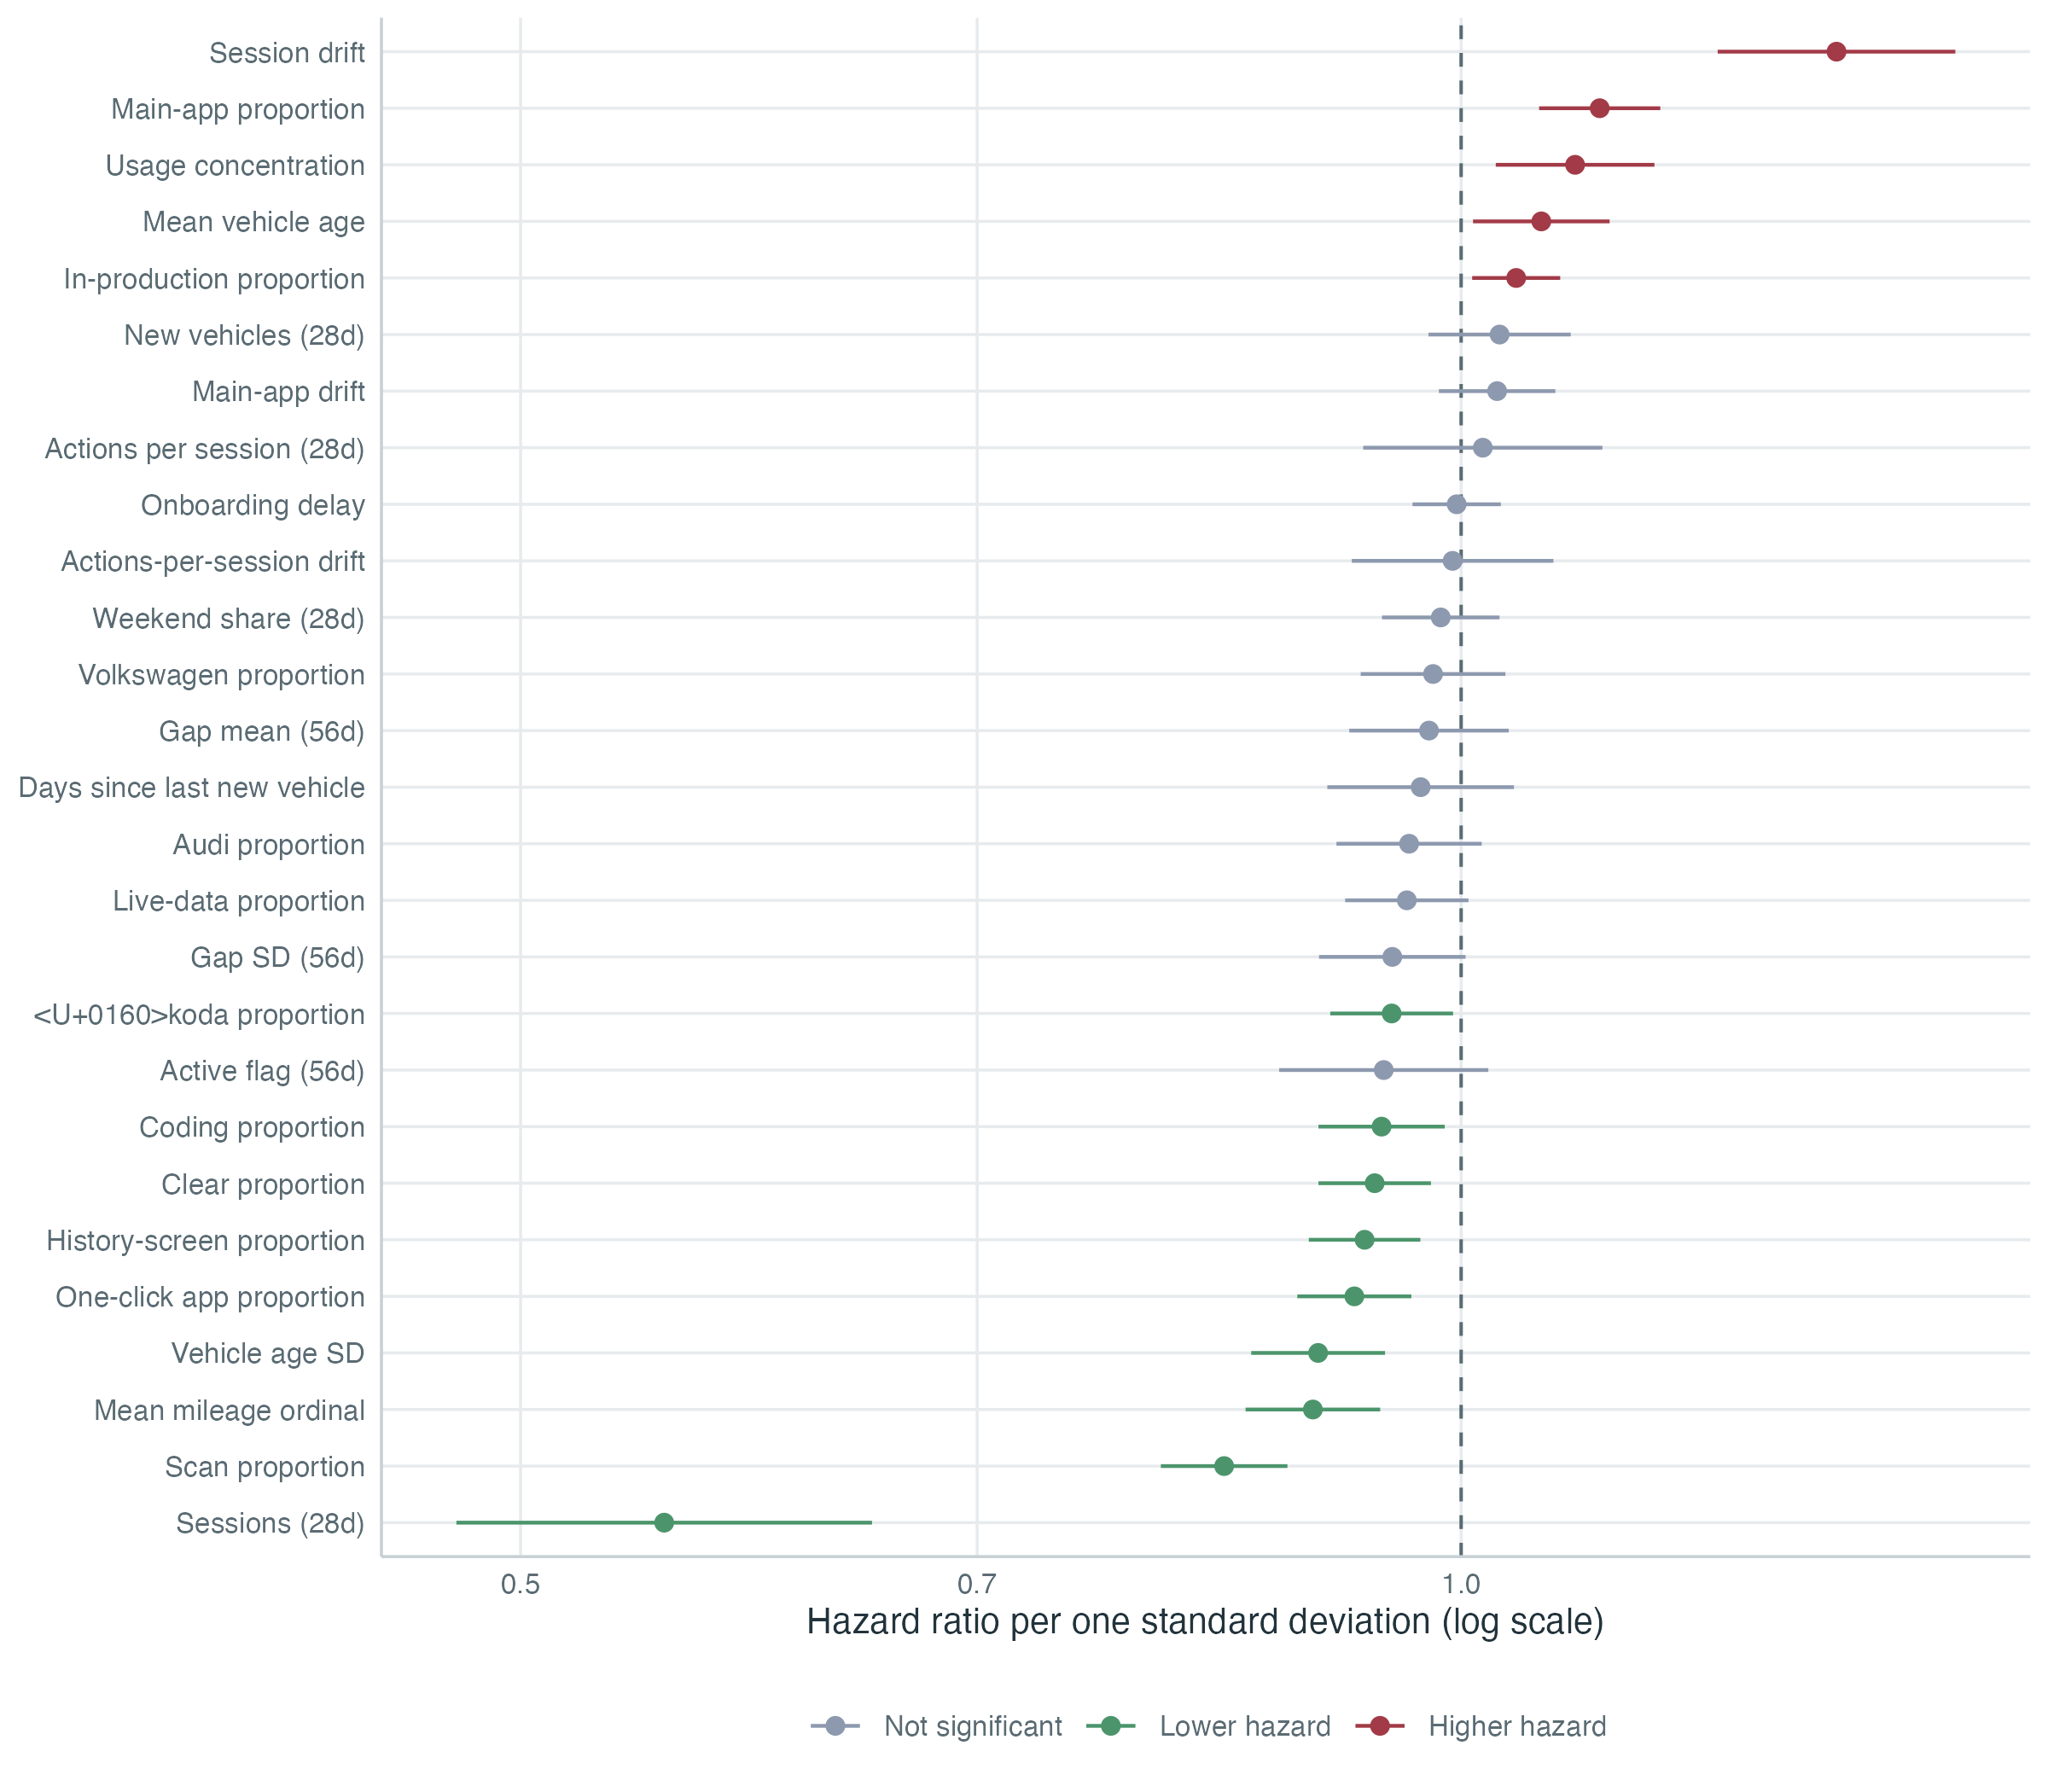
\includegraphics[width=\textwidth]{Images/10_coefficients_m0.png}
\caption{M0 coefficients as hazard ratios per one standard deviation, with 95\% cluster-robust intervals. Intervals crossing 1 are not distinguishable from no effect.}
\label{fig:coefficients}
\end{figure}
 
\begin{table}[htbp]
\centering
\small
\begin{tabular}{@{}lrrrrc@{}}
\toprule
Covariate & $\hat\beta$ & HR per SD & 95\% CI & $p$ & Splined \\
\midrule
Sessions (28d)               & $-0.2025$ & 0.556 & 0.477--0.648 & $<0.001$ & Yes \\
Scan proportion              & $-0.4697$ & 0.840 & 0.801--0.880 & $<0.001$ & Yes \\
Session drift                & $+0.1081$ & 1.319 & 1.208--1.439 & $<0.001$ & Yes \\
Main-app proportion          & $+0.2296$ & 1.108 & 1.059--1.158 & $<0.001$ & Yes \\
Mean mileage ordinal         & $-0.0603$ & 0.896 & 0.853--0.942 & $<0.001$ & Yes \\
Vehicle age SD               & $-0.0444$ & 0.900 & 0.857--0.945 & $<0.001$ & Yes \\
One-click app proportion     & $-0.4374$ & 0.924 & 0.886--0.964 & $<0.001$ & No \\
History-screen proportion    & $-0.5324$ & 0.931 & 0.894--0.970 & 0.001 & No \\
Clear proportion             & $-0.4743$ & 0.938 & 0.900--0.978 & 0.003 & Yes \\
Usage concentration          & $+0.1810$ & 1.088 & 1.026--1.153 & 0.005 & Yes \\
Coding proportion            & $-0.4570$ & 0.943 & 0.900--0.988 & 0.014 & No \\
In-production proportion     & $+0.2678$ & 1.041 & 1.008--1.076 & 0.014 & No \\
Mean vehicle age             & $+0.0135$ & 1.061 & 1.009--1.116 & 0.021 & Yes \\
Škoda proportion             & $-0.2173$ & 0.950 & 0.908--0.994 & 0.027 & No \\
\midrule
Gap SD (56d)                 & $-0.0098$ & 0.951 & 0.901--1.003 & 0.065 & Yes \\
Live-data proportion         & $-0.2257$ & 0.961 & 0.918--1.005 & 0.084 & No \\
Active flag (56d)            & $-0.1167$ & 0.945 & 0.874--1.020 & 0.147 & No \\
Audi proportion              & $-0.1022$ & 0.962 & 0.912--1.015 & 0.160 & Yes \\
Main-app drift               & $+0.0561$ & 1.027 & 0.984--1.072 & 0.226 & Yes \\
New vehicles (28d)           & $+0.0529$ & 1.029 & 0.976--1.084 & 0.289 & No \\
Days since last new vehicle  & $-0.0002$ & 0.971 & 0.906--1.040 & 0.395 & Yes \\
Gap mean (56d)               & $-0.0028$ & 0.977 & 0.921--1.036 & 0.430 & Yes \\
Volkswagen proportion        & $-0.0539$ & 0.980 & 0.929--1.033 & 0.446 & Yes \\
Weekend share (28d)          & $-0.0493$ & 0.985 & 0.943--1.029 & 0.497 & No \\
Actions per session (28d)    & $+0.0096$ & 1.016 & 0.930--1.110 & 0.723 & Yes \\
Onboarding delay             & $-0.00005$ & 0.997 & 0.965--1.030 & 0.843 & Yes \\
Actions-per-session drift    & $-0.0030$ & 0.994 & 0.923--1.070 & 0.868 & Yes \\
\bottomrule
\end{tabular}
\caption{M0 with cluster-robust standard errors, ordered by $p$-value. The rule separates $p<0.05$ from the rest. Hazard ratios are per one standard deviation, because a unit change means the whole range for a proportion and one session for a count. The last column marks the eighteen covariates that enter M1 and M2b as splines.}
\label{tab:coefficients}
\end{table}
 
Fourteen of the twenty-seven covariates reach the 5\% level. Sessions in the trailing 28 days dominates, its test statistic of $-7.5$ just ahead of the scan proportion at $-7.3$. The activity-mix covariates are protective relative to the omitted \emph{other} group, with the main-app and in-production proportions the exceptions. Neither gap covariate reaches significance, although Section~\ref{sec:exclusions} keeps both.
 
Session drift is easily misread. A hazard ratio of 1.32 appears to say that rising activity raises churn. But the 28-day session count sits in the model alongside it, so holding the recent count fixed makes drift a statement about the prior window, where large positive drift means the prior level was low. The coefficient says that a customer at a given current level who arrived there from a lower base carries the higher hazard.
 
% ============================================================
% THE OBDELEVEN PARAGRAPH. Setup written below in the language of the
% four covariate blocks. What is missing is what an operator should do
% with it, which is yours to write.
% ============================================================
Read by block, the pattern is consistent. Volume carries the most weight, with the recent session count the strongest covariate in the model and its drift the third. Activity mix follows, where the diagnostic screens are protective and the main app and in-production screens are not, which separates customers using the product for its core purpose from those browsing it. The fleet block enters through dispersion rather than level, since the spread of vehicle ages and the mileage ordinal both reach the 5\% level while the count of new vehicles does not. The timing block contributes least, with neither gap covariate significant.
 
% [YOUR PARAGRAPH HERE: what OBDeleven should take from this. The
%  reader here is a product owner, not an examiner.]